\documentclass[12pt]{article}
\usepackage{polski}
\usepackage[utf8]{inputenc}
\usepackage{indentfirst} 
\usepackage{hyperref}
\usepackage{geometry}
\usepackage[dvipsnames]{xcolor}
\usepackage[nottoc]{tocbibind}
\usepackage[linesnumbered]{algorithm2e}
\usepackage{textcomp}
\usepackage{listings,chngcntr}
\usepackage{graphicx}
\graphicspath{ {images/} }
\usepackage{float}
\usepackage{caption}

\newtheorem{defin}{Definicja}
\newtheorem{sample}{Przykład}

 
\SetAlgoCaptionLayout{centerline}

\makeatletter
\newcounter{operator}
\newenvironment{operator}[1][htb]
  {
  \renewcommand*{\algorithmcfname}{Operator}%
  \let\c@algocf\c@operator
   \begin{algorithm}[#1]
  }
  {\end{algorithm}}
\makeatother
 
 
\makeatletter
\newcounter{algorytm}
\newenvironment{algorytm}[1][htb]
  {
  \renewcommand*{\algorithmcfname}{Algorytm}%
  \let\c@algocf\c@algorytm
   \begin{algorithm}[#1]
  }
  {\end{algorithm}}
\makeatother

\newcommand{\sectionbreak}{\clearpage}
 \geometry{
 a4paper,
 left=35mm,
 top=25mm,
 bottom=25mm,
 right=25mm,
}

\definecolor{lbcolor}{gray}{0.96}
\lstset{
  backgroundcolor=\color{lbcolor},
  tabsize=4,    
  %   rulecolor=,
  language=[GNU]C++,
  basicstyle=\scriptsize,
  upquote=true,
  aboveskip={1.5\baselineskip},
  columns=fixed,
  showstringspaces=false,
  extendedchars=false,
  breaklines=true,
  prebreak = \raisebox{0ex}[0ex][0ex]{\ensuremath{\hookleftarrow}},
  frame=single,
  numbers=left,
  showtabs=false,
  showspaces=false,
  showstringspaces=false,
  identifierstyle=\ttfamily,
  keywordstyle=\color[rgb]{0,0,1},
  commentstyle=\color[rgb]{0.026,0.112,0.095},
  stringstyle=\color[rgb]{0.627,0.126,0.941},
  numberstyle=\color[rgb]{0.205, 0.142, 0.73}
}
\lstset{
  backgroundcolor=\color{lbcolor},
  tabsize=4,
  language=C++,
  captionpos=b,
  frame=lines,
  numbers=left,
  numberstyle=\tiny,
  numbersep=5pt,
  breaklines=true,
  showstringspaces=false,
  basicstyle=\footnotesize,
  % identifierstyle=\color{magenta},
  keywordstyle=\color[rgb]{0,0,1},
  commentstyle=\color{Darkgreen},
  stringstyle=\color{red}
  keywordstyle = [2]{\color{Violet}},
  keywordstyle = [3]{\color{WildStrawberry}},
  keywordstyle = [4]{\color{Mulberry}},
  otherkeywords = {::,<<,>>,>,<,=,++,--},
  morekeywords = [2]{::},
  morekeywords = [3]{<<, >>, >, <, =},
  morekeywords = [4]{++,--},
}
\def\inline{\lstinline[basicstyle=\ttfamily,keywordstyle={}]}

\begin{document}
\counterwithin{lstlisting}{section}
\begin{titlepage}
	\centering
	{\scshape\LARGE Politechnika Poznańska \par}
	{\scshape\LARGE Wydział Informatyki \par}
	{\scshape\LARGE Instytut Informatyki \par}
	\vspace{1cm}
	{\scshape\Large Praca dyplomowa inżynierska\par}
	\vspace{1.5cm}
	{\huge\bfseries Implementacja algorytmu eksploracji danych z użyciem CUDA API\par}
	\vspace{2cm}
	{\Large\itshape Marcin Jabłoński \par}
	{\Large\itshape Łukasz Kosiak \par}
	{\Large\itshape Piotr Kurzawa \par}
	{\Large\itshape Marek Rydlewski \par}
	\vfill
	\begin{flushright}
	Promotor:\par
	dr inż. ~Witold \textsc{Andrzejewski}
	\end{flushright}
	\vfill
	{\large Poznań, 2017 r.\par}
\end{titlepage}
\thispagestyle{empty} % Strona z pustym stylem, bez numeru
$\mbox{ }$
\vfill\vfill
\hfill
\begin{flushright}
\begin{em}
,,Coś się popsuło`` \\
Zbigniew Stonoga
\end{em}
\end{flushright}
\vfill\pagebreak
\tableofcontents
\newpage

\section{Wstęp}

\subsection{Wprowadzenie}
Informatyzacja życia codziennego, jaka dokonała się w ostatnich latach sprawiła, że każdego dnia konsumenci często nieświadomie zostawiają po sobie wiele informacji na swój temat. Nawet z pozoru niewinne dane o ludzkich przyzwyczajeniach typu "z której półki bierzemy bułki w sklepie" są zapisywane w systemach informatycznych. Należy do tego oczywiście dodać inne usługi, które wybierane są przez użytkowników świadomie np. zapisywanie lokalizacji przez prywatny telefon komórkowy.

Wbrew pozorom, taka błaha na pierwszy rzut oka informacja może mieć jednak istotne znaczenie dla funkcjonowania przemysłu piekarskiego. Nic nie stoi na przeszkodzie, aby spróbować z tych danych odczytać preferencje bądź przyzwyczajenia przeciętnego Kowalskiego na temat jego codziennych zakupów, które mogą w przyszłości zaprocentować - zarówno dla właściciela, jak i klienta. Jest to oczywiście tylko przykład, ale oddaje doskonale fakt przydatności z pozoru nie mających znaczenia prostych czynności człowieka, jakie często przypadkiem rejestrują działające wokół konsumentów systemy.

Pozostaje jednak problem przetworzenia takich danych w celu otrzymania interesującej informacji, która byłaby potencjalnie użyteczna. Trzeba pamiętać, że rozmiar takich danych nierzadko sięga terabajtów i w praktyce skuteczna analiza takich danych przez człowieka nie jest możliwa. Musi on zatem w tym celu skorzystać z dobrodziejstw, jakie przynosi mu współczesna technologia.

Problem efektywnego przetwarzania zdążył urosnąć do rangi oddzielnego działu w informatyce. W pracy \cite{kdd} zasugerowano utworzenie nowej dyscypliny mającej na celu opracowanie technik obliczeniowych rozwiązujących takie problemy, zwanej odkrywaniem wiedzy w bazach danych (ang. KDD – \textit{Knowledge Discovery in Databases}). Techniki te mają na celu odnajdywanie prawidłowych,  nietrywialnych i potencjalnie użytecznych wzorców w dużych zbiorach danych.

Wspominane wyżej techniki w dużej mierze zależą od rodzaju bazy, a ściślej mówiąc - charakteru danych w niej występujących. W przypadku danych zawierających informację o położeniu zazwyczaj mowa jest o  odkrywaniu wiedzy w bazach danych przestrzennych (ang. \textit{spatial data mining}). Takie systemy mogą zawierać atrybut lokalizacji obiektu w danym obszarze, jego opis w formie geometrycznej (np. w postaci wielokątów), a także inne atrybuty nieprzestrzenne. Okazuje się, że tradycyjne metody analizy danych przestrzennych zazwyczaj nie radzą sobie z nimi na tyle efektywnie, by było opłacalne ich użycie w praktyce \cite{trad}, dlatego też zaczęto szukać nowych sposobów na odkrywanie wiedzy w takich bazach.

W pracy \cite{huang} zaproponowano odkrywanie \textit{wzorców kolokacji przestrzennych} (lub krócej: \textit{kolokacji}), czyli zbioru cech przestrzennych występujących w niewielkiej odległości od siebie.  Łatwo to można sobie wyobrazić na przykładzie przyrody, gdzie osobniki (gatunki) o podobnych cechach zazwyczaj trzymają się razem. Rozumowanie to działa również dla bliższych współczesnemu człowiekowi cech przestrzennych, np. punktach o podobnej funkcji - stacje, kina, piekarnie, itd. Wraz z rosnącą popularnością obliczeń na kartach graficznych (w dużej mierze spowodowana wprowadzeniem technologii \textit{CUDA} autorstwa firmy NVIDIA) pojawiło się wiele gotowych rozwiązań, pozwalających na efektywne wyszukiwanie kolokacji nawet w bardzo rozbudowanych bazach danych. Przegląd niektórych z nich można znaleźć w pracy \cite{boinski}.

Ostatni rok przyniósł kolejną metodę efektywnego przeszukiwania baz danych w celu odnalezienia kolokacji \cite{chinczyki}. Wykorzystuje ona autorski algorytm wyszukiwania maksymalnych klik w grafie rzadkim oraz skondensowane drzewa instancji przechowywaczce kliki instancji dla każdego kandydata do kolokacji (patrz Rozdział~\ref{sec:china}) w celu zmniejszenia czasu obliczeń oraz ograniczenia wymagań co do pamięci operacyjnej. Algorytm ten jest przedmiotem badań niniejszej pracy zbiorowej.

\subsection{Cel i zakres pracy}

Celem niniejszej pracy jest analiza wydajności zaproponowanych w pracy \cite{chinczyki} rozwiązań z zakresu odkrywania kolokacji przestrzennych dla GPU i CPU.

Zakres pracy obejmuje następujące zadania szczegółowe:

\begin{enumerate}
\item \textbf{Zapoznanie się z literaturą.} Zapoznanie się z podstawowymi pojęciami dotyczącymi odkrywania danych w bazach danych przestrzennych oraz wyszukiwania wzorców kolokacji przestrzennych jest niezbędne do stworzenia działającej implementacji powyższego algorytmu. Dodatkowo należy zwrócić uwagę na dodatkowe zagadnienia związane z teorią grafów.
\item \textbf{Opracowanie wersji równoległej algorytmu eksploracji danych.} Konieczne jest przemyślenie wykorzystania algorytmów pomocniczych dla poszczególnych kroków całego rozwiązania oraz zaproponowanie możliwie najkorzystniejszego rozwiązania biorąc pod uwagę dostępną pamięć operacyjną, czas przetwarzania i przesyłania danych między pamięcią operacyjną a pamięcią karty graficznej.
\item \textbf{Implementacja wersji sekwencyjnej i równoległej ww. algorytmu.} Rozwiązanie podane w punkcie drugim powinno zostać zaimplementowane w technologii NVIDIA CUDA dla wersji GPU oraz biblioteki PPL w przypadku odmiany dla CPU.
\item \textbf{Przeprowadzenie eksperymentów wydajnościowych.} Analiza wyników testów wydajnościowych implementacji z punktu 3 jest głównym celem tej pracy. Należy zbadać efektywność obu rozwiązań pod względem czasu wykonywania oraz zapotrzebowania na dostępną pamięć. 
\end{enumerate}

\subsection{Charakterystyka źródeł}

Jak już wspomniano, niniejsza praca w dużej mierze opiera się o algorytm zaprezentowany w dokumencie \cite{chinczyki}. Do jej opracowania była wymagana wiedza zawarta w innych źródłach, często również o charakterze naukowym.

Głównym źródłem wiedzy na temat kolokacji przestrzennych była rozprawda doktorska dr inż. Pawła Boińskiego \cite{boinski}, która w dużym przekroju omawia ideę kolokacji zaprezentowaną przez Shekhara i Huanga w pracy \cite{huang}, a także prezentuje najpopularniejsze techniki ich odkrywania (metody \textit{Co-location Miner}, \textit{iCPI-tree}). Część rozwiązań wykorzystanych w tych technikach została wykorzystana w trakcie realizacji algorytmu.

Oddzielną kwestią jest literatura książkowa, wykorzystana do zapoznania się z technologią CUDA oraz przyjęcia dobrych praktyk optymalizacyjnych i programistycznych. Tutaj szczególnie należy wymienić popularną pozycję \textit{CUDA w przykładach} autorstwa Shane'a Cooke'a \cite{cuda_by_examples}, a także \textit{Professional CUDA C Programming} \cite{professional_cuda} będącą również podstawą do wstępu teoretycznego w Rozdziale~\ref{sec:cuda}.

\subsection{Struktura pracy}

\textbf{Rozdział~\ref{sec:theory}} stanowi wstęp teoretyczny do niniejszej pracy - prezentuje podstawowe pojęcia związane z odkrywaniem kolokacji przestrzennych, a także prezentuje najprostsze algorytmy wyszukujące wzorce kolokacji przestrzennych.

\textbf{Rozdział~\ref{sec:cuda}} zawiera wprowadzenie do technologii CUDA. Przedstawia także podstawowe różnice w programowaniu na CPU i GPU oraz wyjaśnia podstawowe pojęcia związane z programowaniem na procesory graficzne.

\textbf{Rozdział~\ref{sec:china}} poświęcony jest algorytmowi \textit{SGCT} będącym głównym tematem pracy. Zawiera wyjaśnienia poszczególnych kroków algorytmu oraz niezbędne definicje.

Implementacja CPU (w wersji sekwencyjnej, jak i równoległej) jest głównym tematem \textbf{Rozdziału~\ref{sec:cpu}}. Koncentruje się on w szczególności na przedstawienie zastosowanych technik optymalizacyjnych poprawiających wydajność algorytmu w środowisku CPU. Rozdział zawiera także krótki wstęp do biblioteki \textit{PPL} użytej w równoległej implementacji algorytmu.

\textbf{Rozdział~\ref{sec:gpu}} zawiera omówienie implementacji algorytmu dla procesorów graficznych (GPU).

Porównanie wydajności zaimplementowanych rozwiązań zostało zawarte w \textbf{Rozdziale~\ref{sec:tests}}. 

Ostatni \textbf{Rozdział~\ref{sec:fin}} stanowi podsumowanie całego projektu, uwagi zespołu oraz możliwe dalsze kierunki rozwoju.

W \textbf{Dodatku~\ref{sec:wypociny}} zawarty jest krótki opis klas zaimplementowanych w implementacji dla CPU i GPU.

\subsection{Podział pracy}

Podział zadań w ramach niniejszego projektu wyglądał następująco:

\begin{itemize}
\item \textbf{Marcin Jabłoński} - równoległa implementacja CPU, testy;
\item \textbf{Łukasz Kosiak} - implementacja GPU, testy;
\item \textbf{Piotr Kurzawa} - tekst pracy inżynierskiej, testy;
\item \textbf{Marek Rydlewski} - sekwencyjna i równoległa implementacja CPU, testy.
\end{itemize}

\newpage

\section{Podstawy teoretyczne}
\label{sec:theory}

\subsection{Charakterystyka danych przestrzennych}

\subsubsection{Modelowanie danych przestrzennych}

Sposób reprezentacji danych przestrzennej w dużej mierze zależy od zastosowań, niemniej najczęściej przybiera jedną z następujących form:

\begin{itemize}
\item \textit{model pól} - ma formę funkcji, której dziedzina należy do modelowanej przestrzeni, a jego wynikiem jest cecha przestrzenna;
\item \textit{model obiektowy} - dla każdego zjawiska jest tworzony nowy obiekt z odpowiednimi właściwościami (etykietami, atrybutami przestrzennymi i nieprzestrzennymi).
\end{itemize}

W praktyce model pól używany jest przede wszystkim w metodach opartych na dokonywaniu pomiarów z powietrza - takie dane mają wtedy charakter rastrowy (reprezentacja w postaci pikseli). Model obiektowy stosowany jest natomiast w przypadkach, gdzie występuje duża liczba dodatkowych atrybutów nieprzestrzennych.

\subsubsection{Źródła danych przestrzennych}

Najogólniej źródła danych przestrzennych można podzielić ze względu na ich format.

\textit{Pierwotne źródła danych} są opracowane w jednym ze standardowych formatów źródeł (najczęściej dla konkretnego systemu) i nie wymagają jakichkolwiek transformacji. Mają one zazwyczaj postać cyfrową i pochodzą z automatycznych pomiarów dokonanych przez specjalizowane systemy wyposażone w odbiorniki GPS czy tachimetry.

\textit{Wtórne dane źródłowe} nie zostały zebrane z myślą o wykorzystaniu w \textit{systemach informacji geograficznej} (ang. \textit{Geographic Information System}, GIS) i dlatego wymagają one odpowiedniej transformacji oraz cyfryzacji (jeżeli są one analogowe). Procedury te są one obarczone pewnym ryzykiem, ponieważ istnieje możliwość wystąpienia błędów w trakcie konwersji i w konsekwencji przekłamaniami w danych wynikowych, które należy ręcznie poprawić.

\subsubsection{Relacje}

Określenie zachodzących relacji między obiektami w źródłach danych przestrzennych jest ważnym elementem przetwarzania danych przestrzennych. Sposób ich określenia zależy od zastosowanego modelu danych.

W modelu pól relacje determinowane są przez operacje pól (ang. \textit{field operations}, \cite{fieldmodel}), mogące przybierać różne formy w zależności od zastosowań, natomiast w modelu obiektowym rodzaje relacji przestrzennych zależą od definicji przestrzeni. Według standardu organizacji OGC (\textit{Open Geospatial Consortium}) istnieją trzy najpopularniejsze rodzaje związków przestrzennych między obiektami:

\begin{itemize}
\item \textit{Relacje metryczne} - wyrażane w postaci predykatów typu "w odległości nie większej niż 10 metrów", oparte na odległości;
\item \textit{Relacje kierunkowe} - położenie określone jest względem globalnych kierunków dla przestrzeni (np. na północ, na południe - są to relacje bezwzględne) lub względem innego obiektu/obserwatora (nazywamy takie relacjami względnymi);
\item \textit{Relacje topologiczne} - najbardziej skomplikowane, wyrażone przez zależności typu pokrywanie, zawieranie, styczność.
\end{itemize}

W systemach typu GIS stosuje się głównie relacje topologiczne. Mają one postać predykatów przestrzennych dla operacji filtrowania i połączenia przestrzennego w językach zapytań działających na danych przestrzennych. Najczęściej wykorzystuje się je w tzw. \textit{modelu dziewięciu przecięć} \cite{9sec}, za pomocą którego określa się możliwe relacje zachodzącą dla pary obiektów.

Dla każdego obiektu wyznacza się jego wnętrze, granicę i zewnętrze. Następnie, dokonuje się operacji przecięcia dla danej pary obiektów dla każdej z możliwych kombinacji elementów tego obiektu (np. granica pierwszego obiektu z wnętrzem drugiego). Takich relacji w dwuwymiarowej relacji można wyznaczyć osiem, należą do nich np. rozłączność, styczność, częściowe i całkowite pokrycie itd. 

Istnieje również rozszerzenie modelu dziewięciu przecięć, zwanym DE-9IM (ang. \textit{Dimensionally Extended nine-Intersection Model}, \cite{9sec2}), które rozróżnia rodzaj obiektu uzyskanego w wyniku przecięcia (mogą być puste, bezwymiarowe, jednowymiarowe i dwuwymiarowe). 

\subsection{Metody eksploracji danych przestrzennych}

Specyfika danych przestrzennych, a w szczególności fakt, że własności obiektu w danych przestrzennych mogą zależeć od cech jego sąsiadów, powoduje, że stosowanie klasycznych metod eksploracji danych może doprowadzić do nieprawidłowych wyników \cite{klasykchuj1} \cite{klasykchuj2} - stąd też istnieje konieczność korzystania z metod eksploracji dedykowanych dla danych przestrzennych. Wiele z nich jest tak naprawdę rozwinięciem metod opracowanych dla klasycznych zbiorów danych.

\subsubsection{Grupowanie przestrzenne}

Metoda grupowania przestrzennego (ang. \textit{spatial clustering}) zakłada istnienie przestrzeni $m$-wymiarowej, w której znajdują się punkty odpowiadające obiektom. Przestrzeń ta ma rozkład niejednorodny, a każdy z obiektów jest opisany przez $m$ atrybutów. Celem grupowania jest poszukiwanie gęstych obszarów punktów używając w tym celu metryki Euklidesowej jako funkcji podobieństwa (bliskości). 

Grupowanie przestrzenne w największym stopniu spośród wszystkich metod eksploracji danych przestrzennych jest podobna do swojego klasycznego odpowiednika - wiele algorytmów grupowania opracowanych dla klasycznych zbiorów danych zadziała również dla danych przestrzennych. 

\subsubsection{Klasyfikacja przestrzenna}

Klasyfikacja przestrzenna (ang. \textit{spatial classification}) działa podobnie jak jego odmiana dla danych klasycznych - przewiduje klasy nowych obiektów w oparciu o tzw. zbiór uczący, składający się ze wcześniejszych obserwacji.

W celu dostosowania klasyfikacji dla danych przestrzennych zaproponowano \cite{klasyfikacja} wykorzystanie \textit{grafu sąsiedztwa} będącego reprezentacją relacji przestrzennych między obiektami, w którym wierzchołki stanowią obiekty przestrzenne, a relacje są krawędziami. Następnie w takim grafie wyznaczane są wszystkie ścieżki, których początkiem jest analizowany obiekt. Dalej analiza przebiega zgodnie z algorytmem \textit{ID3} \cite{id3}.

Z pojęciem klasyfikacji przestrzennej wiąże się także predykcja położenia (ang. \textit{location prediction}), czyli przewidywanie zdarzeń we wskazanym miejscu w przestrzeni, przy uwzględnieniu autokorelacji przestrzennej. Przydaje się ono np. w określaniu regionów o wysokim ryzyku wystąpienia klęsk żywiołowych czy awarii.

\subsubsection{Odkrywanie trendów przestrzennych}

Trend przestrzenny definuje się \cite{toptrendy} jako regularną zmianę co najmniej jednego atrybutu nieprzestrzennego obiektów wraz z oddalaniem się od innego obiektu. Odkrywanie trendów sprowadza się zazwyczaj do analizy regresji, gdzie odległość od danego obiektu jest zmienną niezależną, natomiast różnica wartości atrybutów do obserwacji - zmienną zależną.

Trendy dzieli się na globalne i lokalne. Pierwsze wskazują na zwiększanie (bądź zmniejszanie) wartości obserwowanych atrybutów przy rozpatrywaniu wszystkich obiektów znajdujących się na ścieżkach wychodzących z punktu początkowego. Typowym przykładem jest wzrost bezrobocia wraz z oddalaniem się od centrum miast. Trend lokalny jest reprezentowany przez pojedyncze ścieżki wykazujące inny kierunek zmian na danym atrybucie niż na sąsiednich ścieżkach.

\subsubsection{Przypadki osobliwe w danych przestrzennych}

Czasem w danych przestrzennych można znaleźć obiekty, których atrybuty nieprzestrzenne są niespójne z innymi obserwacjami dokonanymi w ich otoczeniu. Noszą one miano \textit{przypadków osobliwych} \cite{przypadeg}. 

Wyszukiwanie takich zjawisk jest trudne, szczególnie gdy istnieje więcej atrybutów nieprzestrzennych - odwzorowanie ich w $n$-wymiarowej przestrzeni może skutkować \textit{przekleństwem wielowymiarowości} (ang. \textit{curse of dimensionality}) \cite{kurwa}, utrudnionym rozróżnianiem obiektów podobnych do siebie.

\subsubsection{Asocjacje przestrzenne}

Problem odkrywania asocjacji został pierwszy raz zdefiniowany w pracy \cite{asoc} i w ogólności polega na analizie dostępnych transakcji (zbiorów obiektów, np. koszyka zakupów) oraz wykryciu występujących w nich regularności występowania elementów (typu: klient, który kupując bułki wybrał także masło).

Najczęściej reguły charakteryzuje się miarą \textit{wsparcia} (ang. \textit{support}) i \textit{ufności} (ang. \textit{confidence}). Pierwsza z nich wyraża stosunek występowania transakcji zawierającą lewą i prawą stronę reguły do ilości wszystkich transakcji. Ufność z kolei wskazuje na procentowy udział transakcji zawierających lewą i prawą stronę reguły we wszystkich transakcjach, które zawierają jego lewą stronę (jest to tzw. prawdopodobieństwo warunkowe). W celu ograniczenia ilości wykrytych wzorców wprowadzono także pojęcie \textit{zbioru częstego} (ang. \textit{frequent itemsets}) - zbioru elementów, dla których wyznaczone wsparcie przekracza pewien ustalony przez użytkownika próg minimalnego wsparcia. 

Z pracy \cite{asoc} pochodzi także popularny algorytm wykorzystywany w wielu metodach odkrywania asocjacji i kolokacji, czyli metoda \textit{Apriori}. Wykorzystuje on ważną cechę miary wsparcia, jaką jest \textit{antymonotoniczność}. Wynika z niej, że zbiór może być zbiorem częstym tylko w przypadku, kiedy jego podzbiory są również zbiorami częstymi. 

Na początku algorytmu generowane są jednoelementowe zbiory częste. Następnie iteracyjnie wykonywane są następujące kroki:
\begin{itemize}
\item tworzenie zbiorów częstych $ (i + 1) $-elementowych na podstawie zbiorów o długości $ i $,
\item filtrowanie zbiorów kandydujących w oparciu o miarę wsparcia,
\item dodanie kandydatów do zbioru wynikowego.
\end{itemize}

Generowanie kandydatów polega na łączeniu wszystkich par zbiorów częstych o identycznych elementach początkowych, a następnie usuwaniu tych, które nie są zbiorami częstymi w oparciu o własność antymonotoniczności. Algorytm kończy się, gdy zbiór kandydatów będzie pusty.  

W celu dostosowania metody odkrywania asocjacji do danych przestrzennych wprowadzono pojęcie \textit{przestrzennej reguły asocjacyjnej} \cite{asoc2}. Zakłada ona istnienie predykatów przestrzennych (mogących wyrażać informacje o odległości czy kierunku), które mogą występować zarówno w części warunkującej (poprzedniku), jak w warunkowanej (następniku). Następnie podczas procesu odkrywania przestrzennych reguł asocjacyjnych dane umieszczone w ciągłej przestrzeni są zamieniane na zbiór transakcji. Metoda ta jest zaliczana do modelu zorientowanego na cechę referencyjną \cite{boinski}. Istnieje też inne podejście, zwane \textit{odkrywaniem zbiorów częstych klas sąsiadów}, opisane w pracy \cite{classsets}. 

\subsubsection{Kolokacje przestrzenne}

Przedstawiony w pracy \cite{huang} problem \textit{odkrywania przestrzennych reguł kolokacyjnych} powstał w odpowiedzi na niedoskonałości asocjacji (w szczególności konieczność wyboru cechy referencyjnej) i zakłada istnienie równorzędnych cech przestrzennych. 

Praca wprowadza pojęcie \textit{wzorca kolokacji przestrzennej} (zwanego także kolokacją przestrzenną lub krócej - kolokacją), zbioru cech przestrzennych, których instancje często występują we wzajemnym sąsiedztwie \cite{boinski}. Stanowi on swego rodzaju odpowiednik zbiorów częstych w asocjacjach przestrzennych. Również miara wsparcia została zastąpiona przez \textit{miarę powszechności} (ang. prevalence), które eliminują wymaganie wiedzy o transakcjach. 

Kolokacje przestrzenne są przykładem modelu zorientowanego na zdarzenie (ang. \textit{event-centric model}).

\subsection{Odkrywanie kolokacji przestrzennych}

Niniejszy rozdział zawiera opisy i definicje pojęć niezbędnych do zrozumienia algorytmu zawartego w rozdziale 3.

\subsubsection{Cecha przestrzenna}

Kluczową kwestią w procesie odkrywania kolokacji jest odpowiednia klasyfikacja obiektów występujących w bazie danych. Każdy zbiór danych przestrzennych, oprócz informacji o lokalizacji obiektu i opisujących go danych nieprzestrzennych powinien zawierać także właściwość pozwalającą na sklasyfikowanie danego obiektu do określonej klasy. Takie przypisanie nazywane jest cechą przestrzenną (ang. spatial feature) lub rzadziej klasą obiektu (ang. object class).

Jako typowy przykład cechy przestrzennej można podać etykietę przypisaną do obiektu na mapie (np. kosciół, szkoła, strzelnica). Pozwala ona na jednoznaczne określenie własności przestrzeni w punkcie, gdzie znajduje się obiekt.

\subsubsection{Podstawowe definicje}

\begin{defin}[Relacja sąsiedztwa]
Dany jest graf $ G \in (E, V) $. Relacja sąsiedztwa R to relacja istniejąca pomiędzy wierzchołkami w grafie, taka, że jeżeli para (u, v) stanowi krawędź grafu G, to wierzchołek v jest sąsiedni do wierzchołka u. 
\end{defin}

\begin{defin}[Instancja cechy przestrzennej]
Niech f będzie cechą przestrzenną. Mówimy, że obiekt x jest instancją cechy przestrzennej f, wtedy i tylko wtedy, gdy obiekt x jest typu f oraz jest opisany przez lokalizację i identyfikator.
\end{defin}

\begin{defin}[Wzorzec i instancja kolokacji]
Załóżmy $F$ jako zbiór cech przestrzennych $F = \{ f_{1}, f_{2}, ...,f_{m} \} $ , a $FI = FI^{f_{1}} \cup FI^{f_{2}} \cup ... \cup FI^{f_{m}}$ niech będzie
zbiorem ich instancji. Niech $ >_{F} $ oznacza dowolną relację porządku zdefiniowaną dla zbioru $ F $. Niech $ f_{i} $ oznacza i-tą cechę przestrzenną (ze względu na relację $ >_{F} $), zatem $ \forall i,j \in 1,...,m $ $ f_{i} <_{F} $ $ f_{j} \Leftrightarrow i < j \land f_{i},f_{j} \in F $. Mając daną relację sąsiedztwa R (zwrotną i przechodnią) mówimy, że wzorzec kolokacji przestrzennej (w skrócie "kolokacja") jest podzbiorem cech przestrzennych $ c \subseteq F $ , których instancje $ I\subseteq FI $ tworzą klikę ze względu na relację R. Zbiór wszystkich instancji kolokacji przestrzennej $c$ jest oznaczany przez $CI^{c} $. Przez długość kolokacji należy rozumieć liczbę elementów w zbiorze cech przestrzennych, który tworzy tę kolokację.
\end{defin}

\begin{defin}[Sąsiedztwo]
Mające daną zwrotną i symetryczną relację sąsiedztwa R, sąsiedztwem lokalizacji l nazywamy zbiór lokalizacji $L = \{l_{1},l_{2}, . . . , l_{n}\}$, gdzie $l_{i}$ jest sąsiadem l, tzn. zachodzi $R(l, l_{i}) $ $ \forall i \in 1,...,n$.
\end{defin}

Przykład TODO (oprzeć na przykładzie chińczyków?) nk te przykłady

\subsubsection{Miary kolokacji}

\begin{defin}[Współczynnik uczestnictwa]
Współczynnik uczestnictwa (ang. participation ratio) cechy $ f_{i} $ w kolokacji c jest równy procentowemu udziałowi wszystkich instancji cechy $ f_{i} $ w instancjach kolokacji c:

\begin{equation}
pr(f_{i}, c) = \frac{|\pi^{f_{i}}(CI^{c})|}{FI^{f_{i}}}
\end{equation}
gdzie $ \pi^{f_{i}}(CI^{c})$ oznacza projekcję relacyjną zbioru instancji $ CI^{c}$ względem cechy $f_{i}$ (z usuwaniem duplikatów).
\end{defin}

\begin{defin}[Indeks uczestnictwa]Indeks uczestnictwa (ang. participation index) kolokacji c jest równy najmniejszemu ze współczynników uczestnictwa wyznaczonych dla każdej cechy przestrzennej $ f_{i} \in c$:
\begin{equation}
pi(c) = min_{f_{i} \in c} pr(f_{i} ,c)
\end{equation}
Indeks uczestnictwa najczęściej określany jest w literaturze mianem miary powszechności lub krótko powszechnością kolokacji.
\label{def:prevalence}
\end{defin}

\begin{defin}[Maksymalny wzorzec kolokacji przestrzennej]Niech będzie dana wartość min\_prev oznaczająca pewien minimalny próg powszechności. Jeżeli $ c = \{f_{1},...,f_{m} \} $ jest kolokacją powszechną (tzn. $ pi(c) \ge min\_prev $) i nie istnieje żaden nadzbiór c taki, że powszechność dla tego nadzbioru jest równa co najmniej min\_prev, kolokacja c nazywana jest kolokacją maksymalną.  
\end{defin}

\subsubsection{Problem}

%\begin{defin}[Reguła kolokacyjna]Reguła kolokacyjna to reguła postaci $ c_{1} \rightarrow c_{2}(p, cp)$, gdzie $ c_{1} \subseteq F $, $c_{2} \subseteq F $ i $c _{1} \cup c_{2} = \emptyset $. Potencjalna użyteczność reguły może być mierzona przy pomocy jej powszechności p oraz prawdopodobieństwa warunkowego cp.
%\end{defin}

\begin{defin}[Prawdopodobieństwo warunkowe]Prawdopodobieństwem warunkowym
$ cp(c_{1}, c_{2})$ reguły kolokacyjnej $ c_{1} \rightarrow c_{2} $ nazywamy stosunek liczby instancji wzorca c 1 w sąsiedztwie instancji wzorca $ c_{2}$ do liczby wszystkich instancji wzorca $ c_{1} $:
\begin{equation}
cp(c_{1}, c_{2}) = \frac{|\pi^{c_{1}}(CI^{c_{1} \cup c_{2}})|}{CI^{c_{1}}}
\end{equation}
gdzie $\pi^{c_{1}}(CI^{c_{1} \cup c_{2}})$ oznacza projekcję relacyjną instancji wzorca $CI^{c_{1} \cup c_{2}}$ względem wzorca $ c_{1} $ (z usuwaniem duplikatów).
\end{defin}

\begin{defin}[Problem odkrywania kolokacji]
Problem odkrywania kolokacji przestrzennych jest zdefiniowany w następujący sposób.
Mając dane:
\begin{itemize}
\item zbiór cech przestrzennych $F = \{ f_{1}, f_{2}, ...,f_{m} \} $
\item zbiór obiektów $FI = FI^{f_{1}} \cup FI^{f_{2}} \cup ... \cup FI^{f_{m}}$  , gdzie $ FI^{f_{i}},(0 < i \le m) $ jest zbiorem instancji cechy $ f_{i}$, przy czym każda instancja jest opisana przez lokalizację i identyfikator,
\item symetryczną i zwrotną relację sąsiedztwa $R$,
\item próg minimalnej powszechności min\_prev oraz próg minimalnego prawdopodobieństwa warunkowego min\_cond,
\end{itemize}
znajdź wszystkie poprawne reguły kolokacyjne z powszechnością nie mniejszą niż min\_prev i prawdopodobieństwem warunkowym nie mniejszym niż min\_cond.
\end{defin}

\subsection{Przegląd algorytmów odkrywania wzorców kolokacji przestrzennych}

W tym podrozdziale zostaną zaprezentowane skrótowo najważniejsze algorytmy odkrywania kolokacji przestrzennych. 

\subsubsection{Co-location Miner}
\label{subsec:clm}

Wraz z wprowadzeniem pojęcia kolokacji autorzy pracy \cite{huang} zaprezentowali także podstawowy obecnie algorytm rozwiązujący problem odkrywania wzorców kolokacji przestrzennych, zwany \textit{Co-location Miner}. W algorytmie tym wyróżnia się następujące fazy:

\begin{itemize}
\item generowanie kandydatów na kolokacje przestrzenne (o długości $i$),
\item wyznaczanie instancji dla wygenerowanych kandydatów,
\item usuwanie kandydatów, których powszechność wynosi mniej niż przyjęty próg minimalnej powszechności.
\end{itemize}

Pozostali kandydaci trafiają do zbioru wynikowego, a następnie na ich podstawie są tworzone reguły kolokacyjne. Same reguły również podlegają filtracji - usuwane są te reguły, których prawdopodobieństwo warunkowe jest poniżej określonego progu. 

W następnej iteracji algorytm wykonuje dokładnie te same kroki, przy czym generowani kandydaci są o długości o jeden większej. Całość kończy się, gdy nie jest możliwe już wygenerowanie nowych kandydatów.

\subsubsection{Multiresolution Co-location Miner}

Korzystanie z oryginalnego algorytmu \textit{Co-location Miner} wiąże się niestety z dużymi kosztami obliczeniowymi, głównie ze względu na pracochłonny krok generowania kandydatów na kolokacje. Dlatego też niedługo później w pracy \cite{multihuang} autorzy zaproponowali drobną modyfikację oryginalnego algorytmu, dodając dodatkowy krok filtrowania w opraciu o przybliżoną reprezentację zbioru wejściowego.

W algorytmie \textit{Multiresolution Co-location Miner} zbiór wejściowy zostaje podzielony na obszary (mniejsze fragmenty). Zanim rozpocznie się faza wyznaczania instancji dla wygenerowanych kandydatów, nastepuje szacowanie ich powszechności na podstawie sąsiadujących instancji cech przestrzennych w ramach obszarów. W przypadku zbyt niskiej wartości szacowanej powszechności kandydata, można go wykluczyć z dalszego przetwarzania i tym samym oszczędzić zasoby niezbędne na wyznaczenie jego instancji.

Dalsze kroki przebiegają identycznie jak w przypadku oryginalnego \textit{Co-location Miner}.

\subsubsection{Joinless}

Celem autorów pracy \cite{joinless} było stworzenie algorytmu, który omijałby konieczność tworzenia kosztownych połączeń przestrzennych na etapie wyznaczania instancji kandydatów na kolokacje (tak jak np. w przypadku rodziny algorytmów \textit{Co-location Miner}). Nosi on nazwę algorytmu bezpołączeniowego (ang. \textit{joinless}).

Główną różnicą w porównaniu do wcześniejszych algorytmów jest sposób generowania instancji kolokacji. Są one generowane na podstawie sąsiedztw typu gwiazda - zbiorów obiektów, w którego skład wchodzi rozpatrywany obiekt oraz jego sąsiedzi posiadający większą cechę przestrzenną. Wyznacza się je na podstawie oddzielnych algorytmów (np. \textit{plane sweep}), lub korzysta z specjalnych struktur ułatwiających wykrywanie sąsiadów typu \textit{R-drzewo}.

Wygenerowane instancje muszą zostać dodatkowo zweryfikowane (poprawne instancje powinny być kliką, czego nie gwarantuje sąsiedztwo typu gwiazda), a następnie - podobnie jak w algorytmie \textit{Multiresolution Co-location Miner} - dokonuje się ich wstępnego filtrowania pod kątem progu minimalnej powszechności.

\subsubsection{iCPI-tree}

Drzewo iCPI (\textit{improved Co-location Pattern Instance}, \cite{icpi}) stanowi zmodyfikowaną odmianę drzewa CPI zawartego w pracy \cite{cpi}. Struktura ta zawiera informacje o wszystkich zachodzących relacjach sąsiedztwa. 

\textit{iCPI-tree} posiada następującą strukturę:

\begin{itemize}
\item Poziom 1 - korzeń drzewa (oznaczony etykietą \textit{NULL}),
\item Poziom 2 - cechy elementów centralnych, czyli cechy przestrzenne obiektów centralnych \textit{sąsiedztw typu gwiazda};
\item Poziom 3 - instancje elementów centralnych, dla których ma zostać przechowana informacja o sąsiadach;
\item Poziom 4 - cechy sąsiadów,
\item Poziom 5 - instancje sąsiadów.
\end{itemize}

Sąsiedzi uporządkowani są według rosnącej cechy przestrzennej, a w przypadku instancji tej samej cechy - zgodnie z rosnącym identyfikatorem. Takie uporządkowanie nosi nazwę \textit{uporządkowanego zbioru sąsiadów}.

Powyższa struktura drzewiasta jest wykorzystana w algorytmie w celu generowania instancji coraz dłuższych kandydatów w kolejnych iteracjach. Dokonuje się tego poprzez systematyczną ich rozbudowę o kolejne elementy. Na początku wszystkie instancje są jednoelementowe, a w kolejnych iteracjach są one rozbudowywane poprzez wyszukiwanie sąsiadów z odpowiednią cechą i weryfikowane (należy sprawdzić, czy nowo dodany obiekt do instancji jest sąsiadem każdego z obiektów należących do tej instancji). 

Pozostałe kroki algorytmu (generowanie kandydatów i reguł, filtrowanie według powszechności) są podobne jak w metodach \textit{Co-location Miner} i \textit{joinless}.

\newpage

\section{Wprowadzenie do technologii CUDA}
\label{sec:cuda}

Dziedzina informatyki, jaką są obliczenia ogólnego przeznaczenia na układach GPU (ang. \textit{general-purpose computing on graphics processing units}, w skrócie \textit{GPGPU}) należy do stosunkowo świeżych technik programowania - jej właściwy początek można datować na okolice 2007 roku. Jeszcze do niedawna wśród programistów panowało przekonanie, że karty graficzne powinny być odpowiedzialne tylko za rysowanie obrazu, a cała odpowiedzialność za niezbędne obliczenia powinna padać na CPU, jako "serce" komputera. Były to czasy, kiedy pojęcie równoległego wykonywania zadań nie było szeroko rozpowszechnione - rdzenie procesora były jedynie nowinką, a cały rozwój procesorów CPU szedł w zwiększanie częstotliwości taktowania.

Szybko się okazało, że nie da się tego robić w nieskończoność. Podnoszenie częstotliwości spowodowało, że procesory zaczęły pobierać spore ilości energii, a także wydzielać ogromne ilości ciepła, którego nie dało się okiełznać bez korzystania z specjalnego chłodzenia. Rozwiązaniem okazało się skorzystanie z wielordzeniowości - wielu procesorów połączonych ze sobą specjalnymi magistralami, zamkniętymi w jednej obudowie. Wymagało to także zmiany podejścia do programowania. Równoległość daje olbrzymie możliwości, o ile potrafi się z nich skorzystać w odpowiedni sposób - bez tego programista nie uzyska zauważalnego wzrostu szybkości obliczeń, jakie dają współczesne układy wielordzeniowe. 

Wielu osobom w trakcie tej "równoległej rewolucji" umknął pewien fakt - kiedy swoje triumfy świecił procesor \textit{Pentium 4} firmy \textit{Intel} o częstotliwości taktowania rzędu 3 GHz, na rynku istniały już rozwiązania równoległe, na których można było uzyskać znacznie lepsze wyniki. Były to oczywiście karty graficzne, które od dawna działały w sposób równoległy. 

Dopóki nie powstały pierwsze specyfikacje bibliotek wspierających obliczenia na kartach graficznych, programiści próbowali wykorzystywać potencjał brzmiący w procesorach graficznych w oparciu o rendering 3D. Było to dosyć karkołomne zadanie i nie każdy algorytm można było rozwiązać w ten sposób. Karty graficzne musiały odczekać jeszcze parę lat, aby dało się wykorzystać w pełni ich możliwości obliczeniowe.

Spośród wszystkich technologii umożliwiających przeprowadzanie obliczeń na kartach graficznych zdecydowanie największą popularność osiągnęła pierwsza z nich, czyli CUDA (ang. \textit{Compute Unified Device Architecture}). Została ona zaprezentowana po raz pierwszy w 2007 roku przez firmę NVIDIA i jest dedykowana wyłącznie produktom tej firmy (w porównaniu do konkurencyjnej technologii OpenCL).

\subsection{CPU a GPU}

Jak już wspomiano, procesory graficzne, mające w pierwotnym założeniu wyłącznie wspomagać generowanie obrazu, od początku były projektowane jako układy przetwarzajace dane w sposób równoległy. Procesory zawarte w kartach graficznych posiadają znacznie więcej rdzeni niż CPU - mają one jednak mniejsze taktowanie, a także są gorzej wyposażone (w szczególności brakuje im rozszerzeń typowych dla CPU, typu \textit{SSE2} czy \textit{MMX}). W związku z tym, nie wszystkie algorytmy nadają się dobrze do implementacji w środowisku GPU. Jeżeli jednak istnieje możliwość zrównoleglenia jakiegoś problemu zgodnie z paradygmatem SIMD, to wyniki osiągnięte na GPU będą w większości wypadków lepsze niż uzyskane na procesorze CPU. Obecne procesory CPU z kolei potrafią działać sekwencyjnie, jak i równolegle, za pośrednictwem wielu mechanizmów wspierających równoległość (np. wątki, mutexy, wsparcie dla specjalnych struktur).

Oddzielną kwestią jest przydział tranzystorów tworzących poszczególne układy do pełnienia poszczególnych funkcji. W przypadku CPU większość tranzystorów stanowi pamięć podręczną oraz układy sterowania - za wykonywanie obliczeń jest odpowiedzialna ok. 1/4 tranzystorów wbudowanych w procesor. Natomiast w przypadku GPU gros tranzystorów wykorzystanych jest do budowy jednostek arytmetyczno-logicznych oraz zmiennoprzecinkowych. Z tego powodu duża część zadań związana z przepływem danych, uruchamianiem wątków czy podziałem zadań na GPU spoczywa na programiście, co dosyć mocno komplikuje kod.

\subsection{Architektura CUDA}

Procesor graficzny kompatybilny z CUDA zbudowany jest z wielu multiprocesorów strumieniowych (ang. \textit{streaming multiprocessors}, w skrócie SM). Na każdy z nich składa się określona ilość rdzeni CUDA, które mogą przetwarzać dane w sposób równoległy - w każdym z nim jest umieszczona dodatkowo jednostka arytmetyczno-logiczna (ALU, umożliwia obliczenia na liczbach całkowitych) oraz jednostka zmiennoprzecinkowa (FPU). Do tego w każdym \textit{SM} znajdują się jednostki funkcji specjalnych - w nich wyznaczane są wartości funkcji matematycznych typu pierwiastkowanie czy funkcje trygonometryczne. Liczba powyższych elementów nie jest stała - zależą one od miary \textit{potencjału obliczeniowego CUDA} (ang. \textit{CUDA Compute Capability}), który obsługuje dany sprzęt.

Każdy \textit{SM} zawiera 16 jednostek wejścia i wyjścia, mających na celu pośredniczenie w przekazywaniu danych między różnymi typami pamięci. Przez nie odbywa się transfer danych do pamięci RAM karty graficznej (zlokalizowanej poza procesorem graficznym). W multiprocesorze są dostępne następujące typy pamięci podręcznej:

\begin{itemize}
\item pamięć rejestrów - najszybsza pamięć, w której wątek może przechowywać swoje zmienne,
\item pamięć wspólna (ang. \textit{shared memory}) - pamięć, poprzez którą może odbywać się wymiana danych między wątkami;
\item pamięć podręczna pierwszego poziomu (ang. \textit{L1 cache}).
\end{itemize}

Oprócz tego multiprocesor wyposażony jest w układy sterujące wywołaniem instrukcji (ang. \textit{Instruction Dispatch Unit}) odpowiadające za wykonywanie obliczeń na zgrupowanych rdzeniach.

\subsection{Programowanie wielowątkowe w języku CUDA C}

Środowisko programistyczne \textit{CUDA Toolkit} umożliwia programowanie w języku \textit{CUDA C} - stanowi on podzbiór języka C++ i jest z nim w dużym stopniu kompatybilny. Kod w języku \textit{CUDA C} da się łączyć z standardowym kodem C++ kompilowanym pod procesory CPU - w tym przypadku fragmenty kodu wywoływane po stronie karty graficznej są kompilowane przez specjalny kompilator \textit{NVCC} dołączany do środowiska CUDA. 

Funkcje wywoływane przez hosta, a wykonywane przez procesor graficzny w sposób równoległy przez wiele wątków są nazywane funkcjami jądra (ang. kernel). Wszystkie wątki uruchomione poprzez wywołanie jądra wykonują identyczny kod. Oczywiście da się je odróżnić poprzez unikalny identyfikator dostępny w specjalnej zmiennej. Zgodnie z modelem przetwarzania SIMD, na jednym multiprocesorze uruchomione wątki są grupowane w tzw. \textit{warpy} (ang. \textit{warps}) - zbiory 32 wątków wykonujących tą samą instrukcję. 

Wątki można organizować w większe grupy. Podstawową grupą wątków jest \textit{blok}, w ramach którego można uformować wątki w jednym, dwóch, a nawet trzech wymiarach. Bloki grupowane są z kolei w siatkę obliczeniową (ang. \textit{computation grid}), która również może składać się z trzech wymiarów. Przy wywołaniu kernela programista określa liczbę równoległych bloków oraz ilość wątków na blok, za pomocą których urządzenie będzie przetwarzać równolegle kernel. Odpowiednie ustawienie tych wartości jest kluczowe dla wydajności przetwarzania - zbyt mała/wielka ilość przyznanych bloków może spowodować odwrotny skutek do zamierzonego. Maksymalne ilości wątków na blok i bloków na siatkę określa miara \textit{potencjału obliczeniowego CUDA}. 

\subsection{Model pamięci}

Karty graficzne obsługujące technologię CUDA posiadają następujące typy pamięci, dostępne dla programisty:

\begin{itemize}
\item \textit{rejestry} - zdecydowanie najszybsza i najwygodniejsza pamięć, umieszczona w procesorze graficznym, mała, ograniczona żywotność do czasu życia wątku;
\item \textit{pamięć lokalna} - umiejscowiona w pamięci karty graficznej, wolna, będąca alternatywą do rejestrów;
\item \textit{pamięć wspólna} - dostęp do niej możliwy jest ze wszystkich wątków pracujących w ramach jednego bloku, mała (umiejscowiona w chipie GPU), lecz o szybkim czasie dostępu;
\item \textit{pamięć globalna} - duża (rzędu paru gigabajtów), wolna, o dużym czasie dostępu, dostęp z poziomu każdego wątku oraz hosta;
\item \textit{pamięć stała} - dostępna dla wszystkich wątków w trybie tylko do odczytu, buforowana, posiada unikalną możliwość rozgłaszania danych (ang. \textit{broadcast});
\item \textit{pamięć tekstur} - również tylko do odczytu, przeznaczona z myślą o przechowywaniu danych w postaci macierzy.
\end{itemize}

\subsection{\textit{Thrust}}

Biblioteka \textit{Thrust} stanowi odpowiednik popularnej \textit{Standard Template Library} dla języka CUDA C. Od wersji 1.4.0 jego wersja produkcyjna jest dołączana wraz z środowiskiem \textit{CUDA Toolkit 4.0}.

Podobnie jak jego odpowiednik dla języka C++, Thrust zawiera bogatą kolekcję wbudowanych algorytmów i operacji dostosowanych do równoległego środowiska CUDA. W szczególności dostarcza równoległe operacje skanowania, sortowania czy redukcji, zwalniając programistę od implementowania własnych, potencjalnie niewydajnych rozwiązań.

Thrust zawiera struktury znane z biblioteki STL, takie jak wektory (w wersji dla hosta oraz karty graficznej), iteratory oraz wiele innych typów generycznych ułatwiających korzystanie z możliwości dostarczanych przez środowisko CUDA C. Użycie ich jest analogiczne jak w "tradycyjnym" STL-u.

Oprócz tego, biblioteka \textit{Thrust} oferuje następujące operacje:

\begin{itemize}
\item \textit{Inclusive scan} – wyznaczenie tablicy w oparciu o tablicę o rozmiarze k, takiej, że $ B[i] = \sum\limits_{j=0}^{i} A[j], i \in (0, k-1) $;
\item \textit{Exclusive scan} – wyznaczenie tablicy w oparciu o tablicę o rozmiarze k, takiej, że $ B[0] = 0 \cap B[i] = \sum\limits_{j=0}^{i-1} A[j], i \in (1,k-1) $;
\item \textit{Compact} – usuwanie pozycji z tablicy wejściowej spełniającej podany warunek, często na podstawie innej tablicy;
\item \textit{Unique} – wyznaczenie unikalnych wartości z (posortowanej) tablicy wejściowej,
\item \textit{Sort} – sortowanie tablicy podanej na wejściu, również na podstawie klucza sortowania będącego oddzielną tablicą.
\end{itemize}
\newpage

\section{Algorytm \textit{SGCT}}
\label{sec:china}

Niniejszy rozdział ma za zadanie przybliżenie algorytmu będącego tematem tej pracy - metody odkrywania maksymalnych kolokacji przestrzennych w oparciu o graf rzadki i skondensowane drzewo instancji (ang. \textit{sparse-graph and condensed tree-based maximal co-location algorithm}) przedstawionej w pracy \cite{chinczyki}. 

Poszczególne kroki pierwotnego algorytmu \textit{SGCT} zostaną opisane w kolejnych podrozdziałach. Szczegóły implementacji wraz z zaproponowanymi usprawieniami znajdują się w Rozdziale 4.

\subsection{Generowanie tabeli instancji kolokacji o rozmiarze 2}

Pierwszy krok algorytmu jest podobny do metody \textit{Co-location Miner} i polega na wygenerowaniu 2-elementowych kandydatów na kolokacje. 

Kolokacje o rozmiarze 2 tworzone są na podstawie wygenerowanych w oparciu o cechy przestrzenne jednoelementowych kolokacji. Nie jest do tego wykorzystywana jednak metoda \textit{Apriori}, ponieważ udowodniono w pracy \cite{huang}, że dla kandydatów dwuelementowych lepszą wydajność można uzyskać w oparciu o algorytm \textit{spatial join}. Wykorzytany został zatem algorytm \textit{sweeping-based spatial join} \cite{spatial} z dodatkową modyfikacją, usuwającą pary instancji o tej samej cesze przestrzennej. 

\begin{sample}Przykładowe zapytanie tworzące kandydatów na kolokacje o rozmiarze 2 przestawia się następująco:

\textbf{select} $ p', p''$

\textbf{from} $ \{p_{1},...,p_{12}\} p' $, $ \{p_{1},...,p_{12}\} p''$

\textbf{where}  $ p' $.feature $ \neq $ $ p'' $.feature, $ p' \lq p'' $, $(p', p'') \in R$
\end{sample}

Na podstawie wygenerowanych kolokacji oraz tzw. \textit{progu odległości} (ang. \textit{distance threshold}) tworzona jest dwuwymiarowa tablica z haszowaniem (ang. \textit{hash table}). Jest ona indeksowana cechami przestrzennymi. Każdy element tablicy zawiera wskaźnik do listy zawierającej instancje kandydatów o odpowiadających indeksom cechach przestrzennych. Instancja zostanie dodana do tej listy tylko wtedy, gdy odległość między instancjami nie przekracza dopuszczalnego progu odległości między nimi.

%\begin{sample}
%Zapytanie $InsTable_{2}(A,B)$ zwróci listę kandydatów $(A_{2}, B_{2})$, $(A_{3}, B_{1})$, itd. Nie znajdziemy na tej liście pary $(A_{2}, B_{100000})$, gdyż odległość między tymi instancjami przekracza dopuszczalny próg odległości.
%\end{sample}

\subsection{Obliczanie miary powszechności}

Również krok obliczania powszechności dla kandydatów nie różni się od tego znanego z \textit{Co-location Miner}.

Dla każdego kandydata w tabeli wyliczany jest współczynnik uczestnictwa (ang. \textit{participation index}). Dokonuje się tego poprzez wybieranie wszystkich unikalnych instancji cech przestrzennych, która są ujęte w danej kolokacji. Następnie zgodnie z definicją miary powszechności z tabeli instancji są usuwani kandydaci, dla których obliczona miara powszechności jest mniejsza niż zadany próg minimalnej powszechności $ min\_prev $ \cite{huang}. 

\subsection{Generowanie kandydatów na kolokacje maksymalne}

Krok ten wprowadza nową strukturę, zwaną \textit{grafem kolokacji o rozmiarze 2} (ang. \textit{size-2 co-location graph}). Jego definicja brzmi następująco:

\begin{defin}[Graf kolokacji o rozmiarze 2]
Jeżeli przyjąć relacje sąsiedztwa między kolokacjami o rozmiarze 2 jako krawędzie $ E = \{e_{1},...,e_{u}\}$, a cechy przestrzenne występujące w kolokacjach jako wierzchołki $ V = \{v_{1},...,v_{\lambda}\}$, gdzie $ u $ i $ \lambda $ są odpowiednio liczbą krawędzi i liczbą wierzchołków, to graf kolokacji o rozmiarze 2 można zamodelować jako graf nieskierowany $ G= (V, E)$, przechowywany w listowej strukturze danych uporządkowanej rosnąco. Zbiór N jest zbiorem sąsiedztw wierzchołka i definiuje się go następująco:
\begin{equation}
N(v_{i}) = \{W|{v_{i},w} \in E\}
\end{equation}
\label{def:size2-col-graph}
\end{defin}

Zadaniem tego kroku jest wyszukanie w takim grafie maksymalnych klik, określanych jako \textit{kandydaci na maksymalne kolokacje} (ang. \textit{candidate maximal co-location}).

\begin{defin}[Kandydat na maksymalną kolokację]
Kandydat na maksymalną kolokację $ C_{m} $ składa się z uporządkowanych cech przestrzennych o następujących właściwościach: każda para cech w  $ C_{m} $  jest ze sobą połączona krawędzią, a żadne dodatkowe cechy nie mogą być dodane do $ C_{m} $ bez zachowania ich kompletnego połączenia.
\end{defin}

Autorzy pracy \cite{chinczyki} udowodnili, że graf kolokacji o rozmiarze 2 można traktować jako graf rzadki. Umożliwia to efektywne korzystanie z algorytmu Brona-Kerboscha \cite{kerbosz} do wyszukiwania maksymalnych klik w grafie nieskierowanym. Wprowadzone zostały do niego pewne modyfikacje uwzględniające rozproszenie grafu oraz wybieranie \textit{pivotu} w celu usprawienia wyszukiwania kandydatów na kolokacje (patrz Algorytm~\ref{alg:chinczyki_step3}).

\begin{algorytm}

\SetKwInOut{Input}{Wejście}
\SetKwInOut{Output}{Wyjście}
\SetKwProg{myproc}{Procedure}{}{}
\SetKwFunction{proc}{BK\_Pivot}
\Input{$G=(E,V)$}
\Output{$CP_{m}$}
$CP_{m} \leftarrow \emptyset; X \leftarrow \emptyset; P \leftarrow \emptyset$\;
\ForEach{$v^{*}_{i}$ in lista $v^{*}_{1}, v^{*}_{2},..., v^{*}_{\lambda}$  uporządkowanych wg. degeneracji}{
$ P \leftarrow N(V^{*}_{i}) \cup \{ v^{*}_{i+1}, ..., v^{*}_{\lambda}\}$\;
$ X \leftarrow N(V^{*}_{i}) \cup \{ v^{*}_{1}, ..., v^{*}_{i-1}\}$\;
$BK\_Pivot(P,  \{v^{*}_{i}\} ,X)$\;
}

\myproc{\proc{M,K,T}}{
\lIf{$ M \cup T = \emptyset$}{$ \{ CP_{m} \leftarrow CP_{m} \cup K\}$}
wybór $ pivotu $ $ u \in M \cup T ; \% $ do maksymalizacji $ | M \cap N(u) | $\;
\ForEach{$v_{i} \in M \backslash N(u) $}{
$BK\_Pivot(M \cap N(V_{i}), K \cup \{v_{i}\}, T \cap N(V_{i}))$\;
$ M \leftarrow M \backslash \{v_{i}\} $\;
$ T \leftarrow T \cup \{v_{i}\}$\;
}
}
\caption{Generowanie maksymalnych kandydatów na kolokacje}
\label{alg:chinczyki_step3}
\end{algorytm}

Pierwsza z modyfikacji oryginalnego algorytmu dodaje mechanizm \textit{pivoting selection} opisany pierwotnie w pracy \cite{pivot} (linia 9). Jak wykazano w pracy \cite{pivot2} wybranie wierzchołka zmniejszającego liczbę rekurencyjnych wywołań algortytmu znacząco zmniejsza ogólny czas wykonania. Wybiera on wierzchołek będący osią podziału zbioru (tzw. \textit{pivot}) w oparciu o rozmiar unii sąsiadów tego wierzchołka i wierzchołków kandydatów. Każda maksymalna klika musi zawierać albo wierzchołek $ u $, albo niesąsiadujące z nim wierzchołki - jeżeli nie zawiera, zostanie on dodany (linie 11-13). W związku z tym, tylko wierzchołek $ u $ i jego nie-sąsiedzi muszą być przetestowani (linia 10).

Druga modyfikacja opiera się o pojęcie rozproszenia grafu. Opisuje się je miarą \textit{degeneracji grafu} \cite{matusiak}:
\begin{defin}[Degeneracja grafu]
Degeneracja grafu G jest najmniejszą wartością k, taką, że każdy niepusty podgraf G zawiera wierzchołki o stopniu co najwyżej k. Oznacza to, że wielkość maksymalnej kliki nie może przekroczyć $k + 1$.
\label{def:degeneracy}
\end{defin}

\begin{defin}[Uporządkowanie wg. miary degeneracji]
Uporządkowanie według miary degeneracji wierzchołków grafu G to takie uporządkowanie, które minimalizuje stopień degeneracji grafu. Taka uporządkowanie gwarantuje m.in. optymalną kolejność kolorowania w problemie kolorowania wierzchołków.
\end{defin}

Wierzchołki w zewnętrznej rekurencji są uporządkowane według stopnia degeneracji (linia 2). W ciele rekurencji (linie 3-5) liczba wierzchołków czekających na weryfikację nie przekroczy $ k $. Tym sposobem ograniczono liczbę zewnętrznych rekurencji. Dla grafów o małym stopniu degeneracji obserwuje się duży wzrost wydajności \cite{degenerat}.

Autorzy pracy \cite{wang} udowodnili, że zbiór wynikowy kandydatów na kolokacje zawsze będzie zawierał wszystkie maksymalne kliki spełniające próg powszechności. Jest to jeden z warunków poprawności algorytmu generowania maksymalnych kandydatów na kolokacje.

\subsection{Proces odcinania}

W ostatnim kroku w oparciu o tzw. \textit{prunning framework} \cite{wang} nastepuje otrzymywanie końcowych maksymalnych kolokacji spośród kandydatów wyznaczonym w poprzednim procesie. Na początku dla każdego z nich uruchamiany jest algorytm wyszukiwania klik instancji. Do jego zrozumienia niezbędne jest wprowadzenie poniższych definicji.

\begin{defin}[Uporządkowana klika instancji]
Dana jest tabela instancji kolokacji o rozmiarze 2 ($ InsTable_{2}) $ oraz kandydat na maksymalną kolokację $ C_{m} $. Jego uporządkowana klika instancji $ InsC_{m} $ jest grupą instancji przestrzennych spełniających następujące warunki:
\begin{itemize}
\item rozmiar $ InsC_{m} $ jest równy rozmiarowi $ C_{m} $, a cechy w odpowiadających sobie instancjach w $ InsC_{m} $ i $ C_{m} $ są takie same; %a każdej instancji w $ InsC_{m} $ odpowiada cesze w odpowiadającej jej instancji w $ C_{m} $; %
\item instancje każdej pary instancji w $ InsC_{m} $ sąsiadują ze sobą w przestrzeni i można je znaleźć w tabeli  $ InsTable_{2} $.
\end{itemize}
\end{defin}

\begin{defin}[Skondensowane drzewo instancji]Dany jest kandydat na maksymalną kolokację $ C_{m} $. Skondensowane drzewo instancji $ CInsTree$ jest konstrukcją kompresującą wszystkie uporządkowane kliki instancji $ C_{m} $.
\label{def:condensed}
\end{defin}

Algorytm~\ref{alg:chinczyki_step41} ma charakter iteracyjny, w którym zmienna $ i $ jest zmienną sterującą pętli. Na początku zostaje zainicjalizowane drzewo $ CInsTree $ i tworzony jest jego korzeń. Następnie uruchamiany jest proces konstrukcji drzewa, podzielony na dwa etapy. Pierwszy etap wykonywany jest tylko w pierwszej iteracji algorytmu - kolejne iteracje będą wykonywać krok drugi. 

\begin{algorytm}
\SetKwInOut{Input}{Wejście}
\SetKwInOut{Output}{Wyjście}
\SetKwProg{myproc}{Procedure}{}{}
\SetKwFunction{proc}{BK\_Pivot}
\Input{$C_{m}, InsTable_{2}$}
\Output{$CInsTree$ - skondensowane drzewo instancji $ C_{m} $}
$ i \leftarrow 1; CInsTree \leftarrow \emptyset$; utwórz korzeń drzewa $ CInsTree $\;
\While{$ i < size(C_{m}) $}{
	\eIf{$ i = 1 $}{
		\ForEach{para instancji $ InsPair_{k} \in InsTable_{2}(C_{m}(1),C_{m}(2))$}{
			\eIf{$ InsPair(1) \in CInsTree_{0}$.children}{
				dodaj węzeł podrzędny $InsPair_{k}(2)$ do $CInsTree_{1}(InsPair_{k}(1))$\;
			}{
				utwórz poddrzewo z $ InsPair_{k}(1) $ jako korzeniem i $ InsPair_{k}(2) $ jako pierwszym dzieckiem\;
				dołącz to podrzewo do korzenia $ CInsTree $\;
			}
		}
	}{
		\ForEach{węzeł instancji $ ins_{k} \in CInsTree_{i}$}{
			znajdź indeksy elementów równych $ ins_{k} $ od pierwszej kolumny $ InsTable_{2}(C_{m}(i), C_{m}(i + 1))$\;
			przechowaj drugi element odpowiadającej pary instancji w liście $El$\;
			\ForEach{$ei_{t} \in El$}{
				$ flag \leftarrow i - 1 $\;
				$ currIns \leftarrow ins_{k}$.parent\;
				\While{$ flag \geq 1 $}{
					\eIf{$(currInt, ei_{t}) \in InsTable_{2}(C_{m}(flag),C_{m}(i + 1))$}{
						$ currIns \leftarrow currIns$.parent\;
					}{break;}
					$ flag \leftarrow flag - 1 $\;
				}
				\lIf{$ flag = 0 $}{dodaj węzeł podrzędny $ ei_{t}$ do $ CInsTree_{i}(ins_{k})$}
			}
		}
	}			
}
\caption{Konstrukcja skondensowanego drzewa instancji $ C_{m} $}
\label{alg:chinczyki_step41}
\end{algorytm}

W pierwszym kroku (linie 3-11) dla każdej pary instancji pierwszych dwóch cech przestrzennych $ C_{m} $ nastepuje sprawdzenie, czy pierwszy element aktualnie przetwarzanej pary instancji istnieje na danym poziomie drzewa $ CInsTree $ (oznaczonego jako $CInsTree_{1}$). Jeżeli tak, następuje dodanie drugiego elementu jako węzeł podrzędny odpowiadającego mu węzła na poziomie pierwszym. W przeciwnym wypadku, na podstawie obecnej pary instancji tworzone jest poddrzewo, które następnie jest dołączane do korzenia $ CInsTree $. 

Drugi etap rozpoczyna się konstrukcją listy $ El$ zawierającej instancje cechy $ C_{m}(i+1) $. Dokonuje się tego dla każdego węzła instancji na poziomie $i$-tym drzewa $CInsTree$ popzez skanowanie $ InsTable_{2}(C_{m}(i),C_{m}(i+1))$, gdzie $ c_{m}(i)$ jest i-tą cechą $ C_{m} $. Nastepnie dla każdego elementu tej listy nastepuje sprawdzenie, czy zarówno para instancji składająca się z tego elementu, jak i każdy przodek aktualnego węzła instancji $ CInsTree$ znajduje się w tablicy kolokacji o długości 2 - $InsTable_{2}$. Jeżeli tak, dodaje się ten element jako węzeł podrzędny aktualnego węzła instancji.

Proces działa do czasu, gdy nie będzie żadnego węzła na $ i $-tym poziomie drzewa lub dopóki $i$ nie będzie mniejsze niż $ len(C_{m}) - 1 $.

Po zakończeniu algorytmu pozostaje jeszcze wyliczenie indeksów powszechności dla odnalezionych klik instancji. Podobnie jak wcześniej, w przypadku kiedy miara powszechności nie jest mniejsza niż przyjęty na początku próg powszechności, kandydata można przyjąć jako właściwy wzorzec kolokacji \cite{huang}.

\newpage

\section{Implementacja CPU}
\label{sec:cpu}

W tym rozdziale zostaną opisane implementacje rozwiązania problemu \cite{chinczyki} wykorzystujące wyłącznie potencjał procesorów CPU (ang. \textit{Central Procession Unit}), bez udziału karty graficznej w obliczeniach. W szczególności zostaną zaprezentowane techniki optymalizacyjne dedykowane dla poszczególnych podejść do rozwiązania problemu. 

Do celów porównawczych zostały zrealizowane dwa rozwiązania: sekwencyjne (bez żadnego wsparcia dla równoległości) oraz równoległe (z wykorzystaniem biblioteki \textit{Parallel Patterns Library} firmy \textit{Microsoft}). 

\subsection{Wersja sekwencyjna}

\subsubsection{Generowanie instancji w oparciu o próg odległości}
\label{subsec:cpu-step-1}

Podobnie jak w pierwotnej wersji algorytmu, generowanie kandydatów na kolokacje o rozmiarze 2 następuje na podstawie \textit{łączenia przestrzennego w oparciu o zamiatanie} (ang. \textit{sweeping-based spatial join}). Algorytm zamiatania (ang. \textit{plane sweep algorithm}) użyty w procesie łączenia został jednak nieznacznie zmodyfikowany.

Na początku wektor będący zbiorem wejściowym jest traktowany algorytmem \textit{sortowania szybkiego} (ang. \textit{quick sort}) dostępnym w bibliotece standardowej C++. Jako kryterium sortowania zostaje wybrana relacja między arbitralnie wybranym wymiarem przestrzeni.

Następnie następuje wyznaczenie progu odległości, na podstawie którego będą dobierani kandydaci na kolokacje. Warto zwrócić w tym miejscu uwagę na fakt, że algorytmowi nie jest potrzebna wiedza o rzeczywistej odległości między dwoma punktami w przestrzeni, a jedynie relacja między tą odległością a zadanym progiem odległości. Daje to możliwość uniknięcia niepotrzebnych obliczeń (pierwiastkowania) przy wyznaczaniu odlegości między punktami. Dlatego też, zamiast bezpośrednio działać w oparciu o zadany próg odległości, wyliczany jest \textit{efektywny próg odległości}, będącym progiem odległości podniesionym do potęgi drugiej. 

Pozostało już jedynie filtrowanie obiektów w oparciu o wyliczony efektywny próg odległości. Dla każdego obiektu ze zbioru wejściowego następuje przeszukiwanie we wszystkich kierunkach obiektów sąsiadujących z nim, a następnie sprawdzana jest odległość między nimi. Gdy jest ona mniejsza niż ustalony wcześniej próg odległości obiekt umieszczany jest w specjalnej strukturze $ insTable $. Jednocześnie tworzony jest wektor $ typeIncidenceCounter$, w którym zliczane są wystąpienia kolejnych cech instancji przestrzennych (informacja o tym przyda się przy wyznaczaniu miary powszechności). Dodatkowo, pętla wewnętrzna jest przerywana, jeżeli wartość bezwzględna różnicy posortowanych współrzędnych poszczególnych obiektów będzie większa niż zadany próg odległości. Ma to na celu ograniczenie zbędnych porównań w przypadku, kiedy istnieje pewność, że żadne kolejne punkty nie spełnią progu odległości - a zatem nie wejdą do zbioru $ insTable $.
 
Struktura $ insTable $ pełni podobną rolę, jak w oryginalnym algorytmie \textit{SGCT}, nie jest ona jednak dwuwymiarową tablicą z haszowaniem. Zamiast tego zastosowano trójwymiarową mapę wskaźników na wektor liczb, w której wymiarami są kolejno: typ elementu $ A $, typ elementu $ B $ oraz numer instancji przestrzennej $ A $.  W wektorze przechowywane są kolejne numery instancji przestrzennej \textit{B}. W celu efektywnego odczytywania sąsiadów o danej cesze konkretnej instancji, dane w wektorze są umieszczane w taki sposób, że zawsze spełniają relację \textit{numer cechy A} $ > $ \textit{numer cechy B}. Dodatkowo, zamiast standardowej mapy (\textit{std::map}) została wykorzystana mapa nieuporządkowana - gwarantuje ona większą wydajność przeglądania (kosztem większego zużycia pamięci).

\subsubsection{Filtrowanie sąsiadów w oparciu o próg minimalnej powszechności}

Krok ten stanowi zmodyfikowaną wersję algorytmu obliczania miar powszechności znanego z algorytmu \textit{Co-location Miner} (patrz Rozdział~\ref{subsec:clm}).

Na początku wykonywana jest funkcja $ countUniqueInstances$. Ma ona na celu zliczenie wszystkich wystąpień par instancji bez duplikatów. Podobnie jak w kroku pierwszym zostały tu użyte mapy nieuporządkowane (\textit{std::unordered\_map}) w celu przyspieszenia przetwarzania. Do budowy mapy została użyta własna funkcja mieszająca powstała na bazie \textit{hash\_combine} z biblioteki \textit{boost}. Ogranicza ona występowanie kolizji w przypadku wstawiania nowych elementów do tablicy z haszowaniem.

Następnie w oparciu o wektor wynikowy tej funkcji oraz utworzony wcześniej wektor $ typeIncidenceCounter$ (patrz Rozdział~\ref{subsec:cpu-step-1}) dla każdego kandydata w tabeli $ insTable $ wyliczany jest współczynnik uczestnictwa. W przypadku, gdy obliczona miara powszechności jest mniejsza od zadanego progu minimalnej powszechności, kandydat jest usuwany z struktury $ insTable $, a użyta przez niego pamięć zostaje zwolniona na poczet dalszych obliczeń.

\subsubsection{Generowanie kandydatów na kolokacje maksymalne}

Tak jak w przypadku oryginalnego algorytmu, kandydaci na kolokacje maksymalne są generowani w oparciu o \textit{graf kolokacji o rozmiarze 2} (patrz Definicja~\ref{def:size2-col-graph}). Tworzony jest na bazie struktury $ insTable $ za pomocą funkcji \textit{createSize2ColocationsGraph}. Krawędź między elementami pary instancji jest tworzona tylko i wyłącznie wtedy, kiedy numer instancji przestrzennej $ A $ jest większy od zera. 

\begin{algorytm}
\SetKwInOut{Input}{Wejście}
\SetKwInOut{Output}{Wyjście}
\Input{$G=(E,V)$}
\Output{$k$ (miara degeneracji), $L$ (lista wierzchołków uporządkowanych według miary degeneracji)}
$L \leftarrow \emptyset$\; 
$D \leftarrow \emptyset$\;
\ForEach{$v_{i} \in G $}{
$D(d_{v}) \leftarrow $ liczba sąsiadów $ v \notin L $ (początkowo równa stopniowi wierzchołka)\;
}
$k \leftarrow 0$\;
\ForEach{$v_{i} \in G $}{
znajdź takie $ i $, dla którego $ D(i) \neq \emptyset $\;
$ k \leftarrow max(k, i)$\;
$ v \leftarrow $ wierzchołek z $ D(i)$\;
$ L \leftarrow \{v\} \cup L $\;
$ D(i) \leftarrow D(i) \backslash \{v\}$\;
\ForEach{$ w \leftarrow $ sąsiedzi $ v \notin L $}{
$ d^{'}_{w} \leftarrow d_{w} - 1$\;
$ D(d_{w}) \leftarrow D(d_{w}) \backslash \{w\}$\;
$ D(d^{'}_{w}) \leftarrow D(d^{'}_{w}) \cup w $\;
}
}
\caption{Obliczanie miary degeneracji metodą Matuli i Becka (1983)}
\label{alg:matusiak}
\end{algorytm}

Po wygenerowaniu grafu liczona jest jego miara degeneracji (patrz Definicja~\ref{def:degeneracy}). W tym celu został wykorzystany Algorytm~\ref{alg:matusiak} zaprezentowany przez Matulę i Becka w pracy \cite{matusiak}. Działa on w czasie wielomianowym, co pozwala na odciążenie CPU. Funkcja zwraca zarówno miarę degeneracji, jak uporządkowany według niej wektor wierzchołków występujących w grafie.

Dalsze kroki algorytmu wykonywane są dla poszczególnych wierzchołków uporządkowanych według miary degeneracji. Podobnie jak w oryginalnym algorytmie z pracy \cite{pivot} tworzone są grupy wierzchołków o niższych i wyższych indeksach, a następnie uruchamiana jest funkcja $ BK\_Pivot $, w której następuje wyszukiwanie maksymalnych klik w oparciu o algorytm Brona-Kerboscha \cite{kerbosz}. 

Aby ograniczyć czas wyszukiwania maksymalnych klik, zostały zastosowane tzw. \textit{wektory sortowane} zamiast zazwyczaj używanych zbiorów (\textit{std::set}) z biblioteki C++. Posiadają one większą wydajność, a do tego pozwalają na skorzystanie z funkcjonalności zarezerwowanej wyłącznie dla zbiorów.

\subsubsection{Generowanie skondensowanych drzew instancji oraz filtrowanie kandydatów na podstawie progu powszechności}

Na początku wszystkie rozważane maksymalne kliki z poprzedniego kroku są umieszczane w specjalnej strukturze $ cliquesToProcess $ będącej trójwymiarowym wektorem, gdzie pierwsza współrzędna stanowi rozmiar kolokacji, a druga o pozycji kliki w kolejce w poszczególnych wierszach. Trzecią współrzędną są oczywiście kolejne elementy danej kliki.

Następnie iteracyjnie przetwarzana jest każda klika, począwszy od największej. Zrezygnowano w tym miejscu z podejścia rekurencyjnego, gdyż prowadziłoby to do niepotrzebnego utrzymywania ogromnego stosu wywołań (ang. \textit{call stack}). W każdej iteracji sprawdzana jest miara powszechności dla kliki instancji - odpowiedzialna jest za to funkcja $ isCliquePrevalent $. 

Wyliczone kliki są umieszczane w obiektach \textit{CliqueContainer} i \textit{LapsedCliqueContainer}. Pełnią one rolę pamięci podręcznej dla powyższych algorytmów. Dzięki temu nie ma potrzeby ponownego przeliczania tych samych klik instancji, co prowadzi do kilkunastokrotnego wzrostu wydajności obliczeń.

Dla klik o długości większej niż 2 tworzone jest skondensowane drzewo instancji (patrz Definicja~\ref{def:condensed}). Implementacja konstrukcji takiego drzewa zasadniczo nie różni się od pierwotnego algorytmu zaprezentowanego w pracy \cite{chinczyki}, zastosowano w nim jednak pewne metody optymalizacyjne - wskaźniki do rodziców w celu ograniczenia przeszukiwań drzewa w dół, użycie wektora zawierającego wskaźniki do liści znajdujących się na ostatnim poziomie drzewa, wskaźniki typu \textit{unique\_ptr} (więcej szczegółów w Dodatku~\ref{sec:wypociny}). Następnie zliczane są wystąpienia instancji w klikach za pomocą odwróconej pętli i na ich podstawie wyliczana jest miara powszechności.

W przypadku, kiedy miara nie jest mniejsza niż przyjęty na początku próg powszechności, kandydat jest dodawany do zbioru rozwiązań. W przeciwnym wypadku do struktury $ cliquesToProcess $ dodawane są podkliki, które również będą rozważane jako potencjalni kandydaci na kolokacje.

\subsection{Wersja wielowątkowa}

Jak już wcześniej wspomniano, rozwiązanie równoległe zostało oparte o multiplatformową, wysokopoziomową bibliotekę \textit{Parallel Patterns Library} firmy \textit{Microsoft}. Została ona pierwszy raz zaprezentowane szerszej publiczności wraz z wydaniem środowiska \textit{Visual Studio 2010} i docelowo ma być konkurencją dla popularnej biblioteki \textit{OpenMP}. 

Cechą charakterystyczną tej biblioteki jest podobieństwo składni do tej z biblioteki standardowej C++ (ang. \textit{C++ Standard Library}). Wykorzystuje też wszystkie właściwości języka C++, jakie przynosi standard C++11 i późniejsze (w tym funkcje \textit{lambda}).

Biblioteka \textit{PPL} wprowadza zbiór obiektów zwanych \textit{kontenerami o dostępie równoległym} (ang. \textit{concurrent containers}). Są to odpowiedniki kontenerów z biblioteki standardowej C++, które cechują się równoległymi wersjami funkcji operujących na kontenerach (np. operacji wstawiania czy usuwania). W zdecydowanej większości przypadków ich użycie nie różni się od wersji sekwencyjnych dostępnych w bibliotece STD - wymagane jest jedynie umieszczenie ich w odpowiednim bloku, np. \textit{parallel\_for}. 

W przypadku, kiedy istnieje potrzeba dostarczenia kopii kontenera dla każdego z wątków (np. żeby nie blokować dostępu innym wątkom do współdzielonego obiektu), istnieje także klasa kontenerów typu \textit{combinable}. Kiedy równoległe przetwarzanie zostanie zakończone, prywatne kopie wygenerowane dla każdego z wątków są wtedy przezroczyście łączone w całość. Oczywiście \textit{PPL} zawiera także tradycyjne metody zapewnienia równoległości w programie, takie jak zadania (ang. \textit{tasks}) oraz klasyczne mutexy.

Zasadniczą różnicą między \textit{PPL} a \textit{OpenMP} jest zastosowanie dynamicznego planisty (ang. \textit{dynamic scheduler}), co pozwala na lepszą optymalizację równoległego przetwarzania w zależności od aktualnie dostępnych zasobów w systemie. Na dynamicznym planiście zyskują szczególnie problemy o charakterze rekurencyjnym (np. algorytmy sortujące czy szeroko wykorzystywane w niniejszej pracy przeszukiwanie danych) \cite{mikromiekki}. Do tego technologia \textit{OpenMP} nie zawiera żadnego mechanizmu anulowania, często wymaganego w algorytmach o charakterze równoległym \cite{stak}.

Powyższe wady środowiska \textit{OpenMP} były powodem, dla których ostatecznie - pomimo ubogiej dokumentacji oraz niskiej popularności -  została wybrana biblioteka \textit{Parallel Patterns Library} jako najbardziej optymalna dla algorytmu \textit{SGCT} będącego tematem tej pracy.

\subsubsection{Generowanie sąsiadów na podstawie progu odległości}

Różnice w równoległej implementacji generowania sąsiadów w stosunku do wersji sekwencyjnej (patrz Rozdział~\ref{subsec:cpu-step-1}) wynikają w dużej mierze z zastosowania alternatywnych struktur dostępnych w ramach biblioteki \textit{Parallel Pattern Library}. 

Dla przykładu, zbiór wejściowy jest sortowany za pomocą wbudowanego w bibliotekę PPL algorytmu \textit{równoległego sortowania buforowanego} (ang. \textit{parallel buffered sort}). Jest to odmiana standardowego sortowania szybkiego wykorzystujące równoległe scalanie (ang. \textit{parallel merge}) w celu zastąpienia pierwotnego kroku dzielenia w algorytmie sortowania szybkiego, którego nie da się zrównoleglić \cite{buffered-sort} - i podobnie jak \textit{quick sort}, po posortowaniu elementy o tej samej wartości mogą nie występować w tej samej kolejności (przykład tzw. \textit{sortowania niestabilnego}). Dla wielu procesorów pozwala osiągnąć większą wydajność niż standardowy \textit{quick sort} (jego złożoność wynosi $ O((n/p)*\log{n}) $ dla $ p $ procesorów). Podejście to wymaga niestety dodatkowej alokacji pamięci o rozmiarze $ O(n) $. 

W procesie filtrowania obiektów na podstawie wyliczonego progu odległości, podobnie jak w wersji sekwencyjnej, tworzona jest tablica asocjacyjna $ insTable $ -  jednak w podejściu równoległym jest ona typu \textit{combinable}. Dzięki temu każdy wątek posiada swoją prywatną kopię tablicy $ insTable $, w której umieszcza przetwarzane przez siebie pary instancji, które nie przekraczają wyliczonego progu efektywnej odległości. Po zakończeniu przetwarzania przez wszystkie wątki lokalne kopie struktury $ insTable $ są łączone w całość poprzez zastosowanie operacji redukcji oraz sumowania wektorów parami, co eliminuje problem współbieżnego dostępu do struktury w środowisku równoległym. Podobnie sytuacja wygląda w przypadku struktury $ typeIncidenceCounter $.

W algorytmie filtrowania został wykorzystany także dynamiczny planista (\textit{auto partitioner}). W przypadku przerwania pętli wewnętrznej algorytmu, planista dynamicznie przydziela bezczynnym wątkom kolejne dane wejściowe niezbędne do dalszego przetwarzania. Po wyjściu z pętli następuje synchronizacja wątków, a tablica $ insTable $ ulega scaleniu.

Poza powyższymi usprawnieniami, ogólny mechanizm oraz struktury zastosowane w kroku pierwszym pozostały właściwie niezmienione w stosunku do wersji sekwencyjnej. 

\subsubsection{Filtrowanie sąsiadów na podstawie progu minimalnej powszechności}

Jedyną różnicą na tym etapie algorytmu w stosunku do odmiany sekwencyjnej jest dodatkowy krok określenia zakresu pracy dla każdego z wątków biorących udział w liczeniu wystąpień par instancji. Odpowidzialna za to jest funkcja $ getWorkloadForInsTable $.

W porównaniu do poprzedniego etapu, wykorzystywany jest statyczny planista (ang. \textit{static-partitioner}) będący odpowiednikiem funkcji \textit{omp parallel for} z biblioteki \textit{OpenMP}. Dzięki temu każdemu wątkowi przydzielana jest stała ilość par instancji do przetworzenia. Liczba ta jest wyznaczana na podstawie rozmiaru tablicy $ insTable $. Daje to pewną oszczędność czasu, gdyż wątki nie tracą czasu na dynamiczne przydzielanie pracy do wykonania.

\subsubsection{Generowanie kandydatów na kolokacje maksymalne}

Zasadniczą zmianą na tym etapie algorytmu jest wprowadzenie równoległej wersji algorytmu \ref{alg:bk3} liczenia maksymalnych klik metodą Brona-Kerboscha \cite{kerbosz}. Korzysta on ponownie z dynamicznego planisty w celu dynamicznego rozdzielenia pracy dla poszczególnych wątków, ponieważ nieznany jest czas wykonywania algorytmu.

Każdy z wątków uruchamia dla swojej puli wierzchołków standardową wersję algorytmu Brona-Kerboscha wykorzystującą tzw. \textit{pivot}. Podejście to może powodować występowanie duplikatów - dlatego też po zakończeniu działani algorytmów zbiór wynikowy rzutowany jest na kontener \textit{std:set}, likwidując tym samym potencjalnie występujące w zbiorze duplikaty. 

Tradycyjnie na końcu lokalne listy maksymalnych klik są scalane w jedną strukturę wynikową za pomocą instrukcji \textit{combinable::combine\_each}.
\begin{algorithm}

\SetKwInOut{Input}{Wejście}
\SetKwInOut{Output}{Wyjście}
\Input{$G=(E,V)$}
$R \leftarrow \emptyset; X \leftarrow \emptyset; P \leftarrow V(G)$\;
\ForEach{$v^{*}_{i}$ in lista $v^{*}_{1}, v^{*}_{2},..., v^{*}_{\lambda}$  uporządkowanych wg. degeneracji}{
$BK\_Pivot( R \cup \{ v^{*}_{i}\}, P \cap N(v^{*}_{i}), X \cup N(v^{*}_{i})$\;
$ P \leftarrow P \backslash \{v^{*}_{i}\} $\;
$ X \leftarrow X \cup \{ v^{*}_{i}\} $\;
}
\caption{Równoległy algorytm Brona-Kerboscha}
\label{alg:bk3}
\end{algorithm}

 
\subsubsection{Generowanie skondensowanych drzew instancji oraz filtrowanie kandydatów na podstawie progu powszechności}

W porównaniu do wersji sekwencyjnej, konstrukcja skondensowanego drzewa instancji oraz liczenie miary powszechności jest dokonywany w sposób równoległy. Wymagało to zaprojektowania równoległych odpowiedników kontenerów znanych z odmiany sekwencyjnej, czyli \textit{ParallelCliqueContainer} i \textit{ParallelLapsedCliqueContainer} zapewniających bezpieczeństwo przetwarzania rownoległego. Niezbędne było także zastosowanie (podobnie jak w kroku pierwszym) dynamicznego planisty (ang. \textit{auto scheduler}) przydzielającego dynamicznie kolejne kliki do przetworzenia do poszczególnych wątków. Niemożliwe było zastosowanie statycznego planisty z uwagi na fakt, że na tym etapie nie można przewidzieć dokładnego czasu konstrukcji skondensowanego drzewa instancji.

Oddzielną kwestią jest struktura tablicy $ insTable $. Podobnie jak w wersji sekwencyjnej zawiera trzy wymiary. Wykorzystano wektor pochodzący z standardowej biblioteki C++, którego elementy są wskaźnikami na wektory równoległe (ang. \textit{concurrent vector}) pochodzące z biblioteki \textit{PPL} - same z kolei zawierają wskaźniki na wektory klasyczne. To nieco pokrętne rozwiązanie zapewnia bezproblemowe przetwarzanie równoległe, a także - ze względu na minimalizację fragmentacji zaalokowanej pamięci - przyspiesza działanie algorytmu.

Podobnie jak w innych krokach, również tutaj wykorzystywany jest wektor typu \textit{combinable}. Umieszczany jest w niej ostateczny wynik przetwarzania będący scaleniem lokalnych kopii tablic posiadanych przez każdy wątek, biorący udział w wyznaczaniu ostatecznych kandydatów na kololacje.

\newpage

\section{Implementacja GPU}
\label{sec:gpu}
W tym rozdziale zostaną opisane poszczególne kroki implementacji algorytmu wyszukiwania maksymalnych prewalentnych kolokacji przy wykorzystaniu procesorów CUDA. 

Przedstawiona tu implementacja jest silnie zależna od założonej wersji \textit{compute capability} równej 3.0. W wersji tej nie jest dostępna pamięć współdzielona (\textit{Unified Memory}\cite{cuda_um}) oraz \textit{Dynamic Parallelism}\cite{cuda_dp}.

\subsubsection{Przygotowanie danych w pamięci GPU}

Z powodu rozdzielnego modelu pamięci (co zmienia się wraz z wprowadzeniem \textit{unified memory}) dane które zostały wczytane z zewnętrznego źródła (zbiór instancji zawierających typ, identyfikator, położenie w przestrzeni dwuwymiarowej) (//TODO napisać gdzieś o możliwościach rozszerzenia algorytmu) muszą zostać przekazane do pamięci dostępnej dla procesorów CUDA. Operacja przenoszenia danych pomiędzy przestrzeniami pamięci jest dość kosztowna i silnie zależy od wybranych rozwiązań sprzętowych.

\subsubsection{Generowanie tabeli instancji o rozmiarze 2}

Na wejściu tego kroku oczekujemy wczytanej tablicy danych o rozmiarze \textit{n}\textsubscript{dt} zawierającej instancje \{ a\textsubscript{0}, a\textsubscript{1},...,a\textsubscript{\textit{n}\textsubscript{dt} - 1} \} oraz parametru \textit{distanceTreshold} zawierającego wartość maksymalnej odległości pomiędzy instancjami dla których ma zostać stwierdzona relacja sąsiedztwa. Na wyjściu otrzymujemy dwie tablice przechowujące znalezione pary instancji \textit{Pairs}\textsubscript{A} oraz \textit{Pairs}\textsubscript{B}


Algorytm wybrany do rozwiązania tego zadania to algorytm \textit{Planesweep} przystosowany do uruchamiania w architekturze masowo równoległej. Sam algorytm podzielić możemy na dwie części, wyznaczanie ilości sąsiadów dla każdej instancji (kernel \textit{countNeighbours}), a następnie alokacja i wpisanie znalezionych sąsiadów (kernel \textit{findNeighbours}) do tabel \textit{InstanceFirst} oraz \textit{InstanceSecond} które służą do przechowywania par instancji będących w relacji sąsiedztwa, gdzie pierwsza tabela zawiera elementy będące pierwsze w parze, a druga drugie. Wartości należące do jednej pary znajdują się pod tymi samymi indeksami. Kolejność w obrębie pary wyznaczana jest przez następujący operator.

\begin{algorytm}
\SetKwInOut{Input}{Wejście}
\SetKwInOut{Output}{Wyjście}
\SetKwProg{myproc}{Procedure}{}{}
\SetKwFunction{proc}{operator\<}
\Input{$a,b - instancje\ typu\ FeatureInstance $}
\Output{$ bool $}
 \Return $ a.field < b.field $ \; 
\caption{Operator mniejszości dla instancji typu FeatureInstance}
\end{algorytm}
 
Przed wykonaniem samego algorytmu sortujemy zbiór danych wejściowych względem osi odciętych w kolejności rosnącej. Dzięki temu ograniczymy obszar przeszukiwań sąsiadów instancji. Użyta została do tego funkcja sortująca zaimplementowana w bibliotece \textit{Thrust}.

Po zakończeniu sortowania przechodzimy do pierwszego kroku algorytmu \textit{Planesweep}. Tworzymy konfiguracje uruchomieniową dla kernel'a \textit{countNeighbours} z ilością wątków równą \textit{n\textsubscript{dt}} * 32, co daje nam jeden \textit{warp} na instancje. Dodatkowo musimy zaalokować także tablicę \textit{T\textsubscript{counts}} wielkości \textit{n\textsubscript{dt}} w którą na pozycji \textit{i} zostanie wpisana ilość sąsiadów instancji a\textsubscript{i}. Po przygotowaniu danych uruchamiany jest kernel. Każdy warp wykonuje maksymalnie $\lceil i / 32\rceil - 1$ iteracji, w każdej \textit{j-tej} iteracji sprawdzana jest grupa 32 instancji z zakresu K=\{i - j * 32; i - (j + 1) * 32\}. Sprawdzenie polega na obliczeniu odległości euklidesowej pomiędzy instancjami a\textsubscript{i} oraz a\textsubscript{k} i jeśli jest ona nie większa od założonej maksymalnej odległości pomiędzy instancjami \textit{distanceTreshold} stwierdzenie pomiędzy nimi relacji sąsiedztwa . Każdy wątek \textit{warp}'u sumuje w tablicy pamięci współdzielonej ilość znalezionych we wszystkich iteracjach sąsiadów, suma ta jest przechowywana przez każdy wątek w osobnej komórce (pozwala to uniknąć stosowania kosztownego mechanizmu synchronizacji zapisu pomiędzy wątkami \textit{warp}'a). Po każdej iteracji sprawdzane jest czy którykolwiek z wątków \textit{warp}'a napotkał instancje która odległa jest na samej osi odciętych o więcej niż odległość \textit{distanceTreshold}, jeśli tak to można przerwać iterowanie po instancjach, ponieważ korzystając z faktu iż zbiór danych został posortowany po tej osi, nie znajdziemy dalej już żadnych instancji leżących nie dalej niż założony \textit{distanceTreshold}. Po zakończeniu iterowania każdy \textit{warp} wykonuje szybką redukcje części tablicy współdzielonej należącej do jego wątków, a wynik wpisuje do tablicy \textit{T\textsubscript{counts}} na pozycji i.

\begin{figure}[H]
\centering
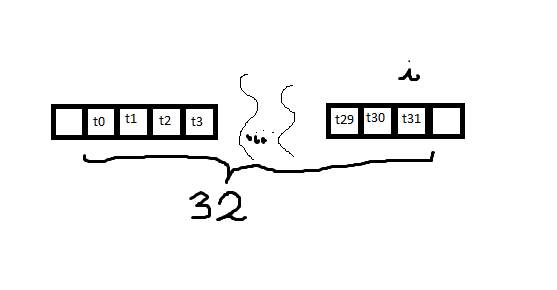
\includegraphics{planesweep}
\caption{Poglądowy rysunek przedstawiający iterowanie warpa po instancjach}
\end{figure}

Po wykonaniu kernel'a \textit{countNeighbours} redukujemy tablicę \textit{T\textsubscript{counts}} otrzymując całkowitą ilość znalezionych relacji sąsiedztwa wśród wszystkich instancji, oznaczmy tę wartość jako \textit{nC}. Alokujemy tablice \textit{Pairs}\textsubscript{A}, \textit{Pairs}\textsubscript{B} każda wielkości \textit{nC}. Dodatkowo alokujemy tablice \textit{Begins} wielkości textit{n\textsubscript{dt}} w której zapisujemy wynik operacji sumy ekskluzywnej tablicy \textit{T\textsubscript{counts}}, która posłuży do wyznaczania pozycji zapisu relacji w tablicach wynikowych.
Konfiguracja uruchomieniowa kernel'a \textit{findNeighbours} jest identyczna z konfiguracją użytą dla \textit{countNeighbours}. Sama funkcja różni się zresztą od poprzedniczki tylko i wyłącznie w miejscu stwierdzenia relacji sąsiedztwa. Mianowicie kernel \textit{findNeighbours} zamiast zliczać relacje sąsiedztwa wpisuje do tablic \textit{Pairs}\textsubscript{A}, \textit{Pairs}\textsubscript{B} instancje pomiędzy którymi ją stwierdzono. Przy pomocy wyżej opisanego operatora mniejszości dla obiektów typu \textit{FeatureInstance} (nie zapisujemy nigdzie informacji o współrzędnych instancji, ponieważ nie będą na dalej nigdzie potrzebne), pozycja zapisu w tablicach wynikowych wyznaczana jest na podstawie wartości w tablicy \textit{Begins} na pozycji \textit{i}, ilości znalezionych przez warp w poprzednich iteracjach relacji sąsiedztwa oraz ilości relacji sąsiedztwa znalezionych w obecnej iteracji przez wątki warpa o mniejszym \textit{id}. Warunki przerwania iterowania są takie same jak w kernel'u \textit{countNeighbours}.

Ostatnią czynnością jest posortowanie par instancji przy użyciu następującego operatora mniejszości

\begin{figure}[H]

\begin{operator}[H]
$operator<(FeatureInstance\ lhs,FeatureInstance\ rhs) $\\
\{\\
  \uIf{$ a[0].fields.featureId\ <\ b[0].fields.featureId $}{
   \Return $ True $ \;
  }\uElseIf { $ a[0].fields.featureId\ ==\ b[0].fields.featureId  $ } {
      \uIf{$ a[1].fields.featureId\ <\ b[1].fields.featureId $}{
   		\Return $ True $ \;
	  }\uElseIf {$ a[1].fields.featureId\ ==\ b[1].fields.featureId $} {
	  	\uIf{$ a[0].fields.instanceId\ <\ b[0].fields.instanceId $}{
   			\Return $ True $ \;
	  	}\uElseIf {$ a[0].fields.instanceId\ ==\ b[0].fields.instanceId $} {
	  		\Return $ a[1].fields.instanceId\ ==\ b[1].fields.instanceId $ \;
	  	}	
	  }
  }
  
  \Return $ False $ \;
\}
  
\caption{Operator mniejszości dla par instancji typu FeatureInstance}
\end{operator}
\end{figure}


Przyczyna takiego uporządkowania zostanie wyjaśniona w kolejnych punktach opisu algorytmu.

\subsubsection{Przygotowanie struktury szybkiego dostępu do informacji o instancjach należących do relacji o zadanych typach }

W tym kroku utworzona zostanie struktura \textit{ITMPack} (opisana w dodatku A), która potrzebna nam będzie w kolejnym kroku. Na wejściu przyjmujemy tablice \textit{Pairs}\textsubscript{A} oraz \textit{Pairs}\textsubscript{B}, wynikiem działania jest struktura ITMPack.

Krok ten korzysta z wprowadzonego w pierwszym kroku uporządkowania zbioru mającego tę właściwość, iż wszystkie relacje o tych samych typach zajmują w wejściowych tablicach ciągły obszar. Przykładowe wartości zaprezentowane zostały na poniższym rysunku

\begin{figure}[H]
\centering
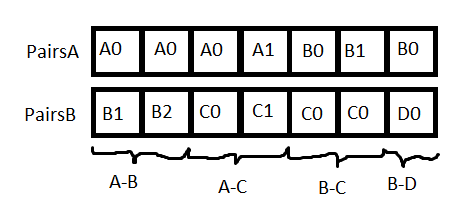
\includegraphics{sortAttr_insTable}
\caption{Przykładowa zawartość tablic \textit{Pairs}\textsubscript{A} oraz \textit{Pairs}\textsubscript{A}}
\end{figure}

Dzięki tej właściwości możemy użyć szybkiego wyznaczenia liczności unikalnych, następujących po sobie elementów. Funkcja ta została zaimplementowana w bibliotece \textit{Thrust} pod nazwą \textit{reduce\_by\_key}. Jako że w tym przypadku instancje są nierozróżnialne względem wartości ich identyfikatorów instancji, a tylko względem identyfikatorów typów użyty został następujący operator relacji równości

\begin{figure}[H]

\begin{operator}[H]
$operator==(FeatureInstanceTuple\ lhs,FeatureInstanceTuple\ rhs) $\\
\{\\
\Return $lhs.get[0].fields.featureId\ ==\ rhs.get[0].fields.featureId$\\
$\ \&\&\ lhs.get[0].fields.featureId\ ==\ rhs.get[0].fields.featureId$\\
\}
\caption{Operator równości dla par instancji typu FeatureInstanceTuple }
\end{operator}
\end{figure}

Gdzie \textit{FeatureInstanceTuple} to obiekt typu para dwóch obiektów \textit{FeatureInstance}, czyli obiekt łączący elementy z tablicy \textit{Pairs}\textsubscript{A} z odpowiadającymi im pozycją elementami tablicy \textit{Pairs}\textsubscript{B}.
Wynikiem działania funkcji \textit{reduce\_by\_key} są trzy tablice o jednakowym rozmiarze \textit{c\textsubscript{r}}
\begin{itemize}
\item \textit{Uniques} zawierająca pary typów dla których istnieje przynajmniej jedna para instancji
\item \textit{Counts} zawierającą liczności instancji relacji dla par typów instancji
\item \textit{Begins} zawierająca indeksy tabeli instancji relacji oznaczające początki obszarów ciągłych odpowiadającym danym parom typów instancji
\end{itemize}

Tablice te są częścią struktury \textit{ITMPack}. Na podstawie tych danych uzupełniana jest mapa struktury \textit{ITMPack}, służy do tego kernel uruchamiany z ilością wątków równym \textit{c\textsubscript{r}}, który dla każdego \textit{i}-tego elementu tablic tworzy strukturę \textit{InstanceTable} uzupełniając ją \textit{i}-tymi wartościami z \textit{Counts} oraz \textit{Begins}, a następnie wstawia go do tablicy pod kluczem utworzonym z \textit{i}-tego elementu tablicy \textit{Uniques} (klucz ten ma postać połączonej pary typów).

Tak uzupełniona struktura \textit{ITMPack} jest wynikiem tego kroku.


\subsubsection{Generowanie prewalentnych relacji sąsiedztwa pomiędzy typami połączeń}

W tym kroku wyznaczane są prewalentne pary typów czyli takie których współczynnik powszechności jest nie mniejszy niż zadany próg powszechności.

Na wejściu wymagane jest podanie informacji o liczności poszczególnych typów, wygenerowanych instancji relacji sąsiedztwa oraz struktury \textit{ITMPack} 
Na wyjściu otrzymujemy listę prewalentnych par typów na podstawie których w kolejnym kroku utworzony zostanie graf do generowania kandydatów klik maksymalnych.

Na początku tego kroku tworzymy dwie tablice, \textit{countsA} oraz \textit{countsB}, każda z nich rozmiaru tablicy \textit{ITMPack}.\textit{uniques}.
W celu uzupełnienia tablicy \textit{countsA} dla każdego elementu tablicy \textit{ITMPack}.\textit{uniques} pobieramy 


\newpage
\section{Testy efektywnościowe}
\label{sec:tests}

\section{Zakończenie}
\label{sec:fin}

\newpage

\begin{thebibliography}{}
% Autorzy, Tytuł, Gdzie ?, Rok wydania, Strony
\bibitem{kdd}Usama Fayyad, Gregory Piatetsky-Shapiro, and Padhraic Smyth. From Data Mining to Knowledge Discovery in Databases. AI Magazine, 17:37–54, 1996.
\bibitem{trad} Harvey J. Miller and Jiawei Han. Geographic Data Mining and Knowledge Discovery.
Taylor \& Francis, Inc., Bristol, PA, USA, 2001
\bibitem{huang} S. Shekhar and Y. Huang. Discovering Spatial Co-location Patterns: A Summary of Results. In SSTD 2001, pages 236–256, 2001.
\bibitem{boinski} Boiński P., Przetwarzanie zbiorów przestrzennych zapytań eksploracyjnych w środowiskach z ograniczonym rozmiarem pamięci operacyjnej, Poznań, 2015.
\bibitem{chinczyki}Yao X., Peng L., Yang L., Chi T. A fast space-saving algorithm for maximal co-location pattern mining. W: Expert Systems with Applications Volume 63, 30 November 2016, strony 310–323.
\bibitem{cuda_by_examples}Sanders J., Kandrot E., CUDA by Example: An Introduction to General-Purpose GPU Programming, Addison-Wesley, 2011.
\bibitem{professional_cuda}Cheng J., Grossman M., McKerche T. Professional CUDA C Programming, Wrox, 2014.
\bibitem{multihuang}Shashi Shekhar and Yan Huang. The Multi-resolution Co-location Miner: A New Algorithm to Find Co-location Patterns in Spatial Dataset. Technical Report 02-019, University of Minnesota, 2002.
\bibitem{joinless}Jin Soung Yoo and Shashi Shekhar. A Joinless Approach for Mining Spatial Colocation Patterns. IEEE Transactions on Knowledge and Data Engineering, 18(10):13231337, 2006.
\bibitem{cpi}Lizhen Wang, Yuzhen Bao, Joan Lu, and Jim Yip. A New Join-less Approach for Co-location Pattern Mining. In Qiang Wu, Xiangjian He, Quang Vinh Nguyen, Wenjing Jia, and Mao Lin Huang, editors, Proceedings of the 8th IEEE International
Conference on Computer and Information Technology (CIT 2008), pages 197–202, Sydney, July 2008. IEEE.
\bibitem{icpi}Lizhen Wang, Yuzhen Bao, and Joan Lu. Efficient Discovery of Spatial Co-Location Patterns Using the iCPI-tree. The Open Information Systems Journal, 3(2):69–80,2009.
\bibitem{fieldmodel}Christopher Jones and Mark Hall. A Field Based Representation for Vague Areas Defined by Spatial Prepositions. In Proceedings of the Workshop on Methodologies and Resources for Processing Spatial Language at 6th Language Resources and Evaluation Conference (LREC 2008), 2008.
\bibitem{9sec}Max J. Egenhofer and Robert Franzosa. Point-set topological spatial relations. International Journal of Geographic Information Systems, 5(2):161–174, 1991.
\bibitem{9sec2} Eliseo Clementini, Paolino Di Felice, and Peter van Oosterom. A small set of formal topological relationships suitable for end-user interaction. In Proceedings of the 3rd International Symposium on Advances in Spatial Databases (SSD 1993), pages 277-295, London, UK, UK, 1993. Springer-Verlag.
\bibitem{klasykchuj1} Harvey J. Miller and Jiawei Han. Geographic Data Mining and Knowledge Discovery. Taylor \& Francis, Inc., Bristol, PA, USA, 2001.
\bibitem{klasykchuj2}John F. Roddick and Myra Spiliopoulou. A Bibliography of Temporal, Spatial and Spatio-Temporal data Mining Research. ACM SIGKDD Exploration Newsletter, 1(1):34–38, 1999.
\bibitem{klasyfikacja}Martin Ester, Hans-Peter Kriegel, and Jörg Sander. Spatial Data Mining: A Database Approach. In Proceedings of the 5th International Symposium on Advances in Spatial Databases (SSD 1997), pages 47–66, London, UK, UK, 1997. Springer-Verlag.
\bibitem{id3} John R. Quinlan. Induction of Decision Trees. Machine Learning, 1(1):81–106, March 1986.
\bibitem{toptrendy}Martin Ester, Alexander Frommelt, Hans-Peter Kriegel, and Jörg Sander. Algorithms for characterization and trend detection in spatial databases. In Proceedings of the 4th International Conference on Knowledge Discovery and Data Mining (KDD 1998), pages 44–50, 1998.
\bibitem{przypadeg}Shashi Shekhar and Sanjay Chawla. Spatial Databases: A Tour. Prentice Hall, 2003
\bibitem{kurwa} Richard E. Bellman. Adaptive control processes - A guided tour. Princeton University Press, Princeton, New Jersey, U.S.A., 1961.
\bibitem{asoc} Rakesh Agrawal and Ramakrishnan Srikant. Fast Algorithms for Mining Association Rules in Large Databases. In Proceedings of the 20th International Conference on Very Large Data Bases (VLDB 1994), pages 487–499, San Francisco, 1994. Morgan Kaufmann Publishers Inc.
\bibitem{asoc2} Krzysztof Koperski and Jiawei Han. Discovery of Spatial Association Rules in Geographic Information Databases. In Max J. Egenhofer and John R. Herring, editors, Proceedings of the 4th International Symposium on Advances in Spatial Databases (SSD 1995), volume 951 of Lecture Notes in Computer Science, pages 47–66. Springer Berlin Heidelberg, 1995
\bibitem{classsets}Yasuhiko Morimoto. Mining Frequent Neighboring Class Sets in Spatial Databases. In Proceedings of the 7th ACM SIGKDD International Conference on Knowledge Discovery and Data Mining (KDD 2001), pages 353–358, New York, NY, USA, 2001. ACM.
\bibitem{spatial}L. Arge, O. Procopiuc, S. Ramaswamy, T. Suel, and J. Vitter. Scalable Sweeping-
Based Spatial Join. In Proc. of the Int’l Conference on Very Large Databases, 1998.
\bibitem{degenerat}Eppstein, D. , Löffler, M. , i Strash, D. (2010). Listing all maximal cliques in sparsegraphs in near-optimal time. In O. Cheong, K. Y. Chwa, \& K. Park (Eds.), 21st international symposium on algorithms and computation (pp. 403–414). Berlin, Germany: Springer-Verlag.
\bibitem{kerbosz}Bron, C., \& Kerbosch, J. (1973). Algorithm 457: Finding all cliques of an undirected graph. Communications of the ACM, 16 , 575–577.
\bibitem{pivot}Tomita, E., Tanaka, A., \& Takahashi, H. (2006). The worst-case time complexity for
generating all maximal cliques and computational experiments. Theoretical Computer Science, 363 , 28–42.
\bibitem{pivot2}Cazals, F.; Karande, C. (2008), "A note on the problem of reporting maximal cliques" , Theoretical Computer Science, 407 (1): 564–568.
\bibitem{wang}Wang, L., Zhou, L., Lu, J., \& Yip, J. (2009). An order-clique-based approach for mining maximal co-locations. Information Sciences, 179 , 3370–3382.
\bibitem{matusiak}Matula, D. W.; Beck, L. L. (1983), "Smallest-last ordering and clustering and graph coloring algorithms", Journal of the ACM, 30 (3): 417–427, doi:10.1145/2402.322385, MR 0709826.
\bibitem{mikromiekki}Comparing the Concurrency Runtime to Other Concurrency Models, Microsoft, 2015 [dostęp: 10-01-2017]. Dostępny w Internecie: https://msdn.microsoft.com/en-us/library/dd998048.aspx\#openmp
\bibitem{stak}Microsoft Parallel Patterns Library (PPL) vs. OpenMP, Stack Overflow, 14-03-2012 [dostęp: 10-01-2017]. Dostępny w Internecie: http://stackoverflow.com/questions/9700088/microsoft-parallel-patterns-library-ppl-vs-openmp
\bibitem{cuda_um}https://devblogs.nvidia.com/parallelforall/unified-memory-in-cuda-6
\bibitem{buffered-sort}. Sorting in PPL, Parallel Programming in Native Code, vinodsu (Microsoft Developer Network Blogs), 14-01-2011 [dostęp: 10-01-2017]. Dostępny w internecie: https://blogs.msdn.microsoft.com/nativeconcurrency/2011/01/14/sorting-in-ppl/
\bibitem{cuda_dp}https://devblogs.nvidia.com/parallelforall/cuda-dynamic-parallelism-api-principles

\end{thebibliography}
\newpage

\appendix

\section{Opis klas i struktur pomocniczych}
\label{sec:wypociny}

\subsection{Opis architektury wersji CPU}

Podczas implementacji stworzono dwie główne klasy: CpuMiningAlgorithmSeq oraz CpuMiningAlgorithmParallel dziedziczące po klasie abstrakcyjnej CpuMiningAlgorithmBase. CpuMiningAlgorithmBase zawiera cztery metody czysto wirtualne (ang. \textit{pure virtual functions}) odpowiadające za główne kroki algorytmu:

\begin{itemize}
\item
Filtrowanie sąsiadów na podstawie progu odległości:
\begin{lstlisting}
virtual void filterByDistance(float threshold) = 0;
\end{lstlisting}

\item
Filtrowanie sąsiadów na podstawie progu minimalnej powszechności:
\begin{lstlisting}
virtual void filterByPrevalence(float prevalence) = 0;
\end{lstlisting}

\item
Generowanie kandydatów na kolokacje maksymalne:
\begin{lstlisting}
virtual void constructMaximalCliques() = 0;
\end{lstlisting}

\item
Generowanie skondensowanych drzew instancji kandydatów na kolokacje maksymalne i ich filtrowanie na podstawie progu minimalnej powszechności:
\begin{lstlisting}
virtual std::vector<std::vector<unsigned short>> 
    filterMaximalCliques(float prevalence) = 0;
\end{lstlisting}
\end{itemize}

Klasy CpuMiningAlgorithmSeq oraz CpuMiningAlgorithmParallel zawierają implementację owych metod odpowiednio w wersji sekwencyjnej jak i równoległej.

Oprócz wyżej wspomnianych metod klasa CPUMiningAlgorithmBase zawiera implementację metod pomocniczych odpowiadających za:

\begin{itemize}
\item Obliczenie odległości między instancjami i porównanie ich z obowiązującym progiem odległości.
\item Obliczenie wartości funkcji powszechności dla dwóch elementów.
\item Obliczenie wartości funkcji powszechności dla dowolnej liczby elementów, za równo w wersji sekwencyjnej i równoległej.
\item Wygenerowanie wszystkich podklik kliki K o rozmiarze \textit{n} takich, że rozmiar każdej podkliki wynosi \textit{n - 1}.
\end{itemize}

\subsection{Opis struktur \& klas pomocniczych i ich implementacji}
    
\begin{itemize}
\item DataFeed - Instancje struktury DataFeed mają za zadanie przechowywać dane wejściowe.

\begin{minipage}{\linewidth}
\begin{lstlisting}[caption={Kod struktury DataFeed}]
struct DataFeed
{
    struct Coords
    {
        float x;
        float y;
        Coords(float x, float y) : x(x), y(y) {}
    };
    
	unsigned short type;
	unsigned short instanceId;
	Coords xy;
    
	DataFeed(unsigned short type,
        unsigned short id,
        float x,
        float y)
    		: type(type), instanceId(id), Coords(x,y) {}

	bool operator < (const DataFeed& str) const
	{
		return (type == str.type)?(instanceId < str.instanceId):(type < str.type);
	}
};
\end{lstlisting}
\end{minipage}

\item FeatureInstance - \lstinline{Unia} składająca się z pola typu \lstinline{unsigned int} oraz struktury zawierającej dwa pola typu \lstinline{unsigned short} służąca do przechowywania identyfikatora typu oraz unikalnego względem typu identyfikatora instancji.

\begin{lstlisting}
union __declspec(align(4)) FeatureInstance
{
	unsigned int field;

	struct __inner
	{
		unsigned short instanceId;
		unsigned short featureId;
	} fields;
};
\end{lstlisting}

\item InstanceTable - klasa przetrzymująca informacje o indeksie startowym w tablicach przechowywujących posortowane instancje relacji sąsiedztwa oraz ich ilości. 

\begin{minipage}{\linewidth}
\begin{lstlisting}[caption={Kod klasy InstanceTable}]
	class InstanceTable
	{
	public:
		unsigned int count;
		unsigned int startIdx;
	};
\end{lstlisting}
\end{minipage}

\item ITMPack - struktura przechowująca informacje potrzebne do szybkiego dostępu do wszystkich instancji relacji o zadanych typach (na przykład wszystkich instancji relacji o typach \{A,B\}).

\begin{minipage}{\linewidth}
\begin{lstlisting}[caption={Kod struktury ITMPack}]

	struct ITMPack
	{
		InstanceTableMapPtr map;
		thrust::device_vector<unsigned int> begins;
		thrust::device_vector<unsigned int> counts;
		thrust::device_vector<FeatureInstanceTuple> uniques;
		unsigned int count;
	};
\end{lstlisting}
\end{minipage}

\item CinsTree - Klasa zawierająca implementację skondensowanego drzewa instancji (ang. \textit{condensed instance tree}). Zawiera wskaźnik do korzenia drzewa \raggedright \inline{std::unique_ptr<CinsNode> root}) oraz wektor \inline{std::vector<CinsNode*> lastLevelChildren} zawierający wskaźniki do liści znajdujących się na ostatnim poziomie (wynikającym z rozmiaru aktualnie budowanej kliki - w przypadku gdy nie udało się rozbudować drzewa o kolejny poziom lista ta jest pusta) owego drzewa. Takie podejście umożliwia szybki dostęp do finalnych instancji poszczególnych kandydatów na kolokacje.

\item CinsNode - Klasa zawierająca implementację pojedynczego węzła skondensowanego drzewa instancji \textit{CinsTree}. Obiekty tej klasy zawierają informacje o cesze \inline{unsigned short type} i numerze \inline{unsigned short instanceId} instancji przestrzennej, wektor wskaźników potomków \inline{std::vector<std::unique_ptr<CinsNode>> children} oraz wskaźnik pokazujący na rodzica danego węzła \inline{CinsNode* parent}. Klasa zawiera metody umożliwiające m.in.:

\begin{itemize}
\item dodanie potomka.
\item zwrócenie potomka o danej cesze i numerze instancji.
\item zwrócenie listy wszystkich przodków.
\end{itemize}

\item Graph - Klasa implementująca graf nieskierowany, bazująca na macierzy sąsiedztwa (ang. \textit{adjacency matrix}). Oprócz podstawowych metod umożliwiających działanie i budowanie grafu, klasa zawiera również metody pozwalające na:

\begin{itemize}
\item obliczenie maksymalnych klik w grafie za pomocą zmodyfikowanego algorytmu Brona-Kerboscha \cite{chinczyki}.
\item obliczenie optymalnego \textit{pivotu} \cite{pivot} dla algorytmu Brona-Kerboscha.
\item obliczenie stopnia degeneracji grafu (ang. \textit{degeneracy}) i uporządkowanie wierzchołków według miary degeneracji (ang.\textit{degeneracy ordering}) \cite{degenerat}.
\end{itemize}

\begin{minipage}{\linewidth}
\begin{lstlisting}[caption={Kod metody tomitaMaximalPivot umożliwiającej wyliczenie optymalnego punktu \textit{pivot}}]
unsigned short Graph::tomitaMaximalPivot(
	const std::vector<unsigned short>& SUBG,
    const std::vector<unsigned short>& CAND)
{
	unsigned short u, maxCardinality = 0;
	for (auto s : SUBG)
	{
		auto neighbors = getVertexNeighbours(s);
		std::sort(neighbors.begin(), neighbors.end());
		
		std::vector<unsigned short> nCANDunion(neighbors.size() + CAND.size());
        
		auto itUnion = std::set_union(
        	CAND.begin(),
            CAND.end(),
            neighbors.begin(),
            neighbors.end(),
            nCANDunion.begin());
            
		nCANDunion.resize(itUnion - nCANDunion.begin());
		if (nCANDunion.size() >= maxCardinality)
		{
			u = s;
			maxCardinality = nCANDunion.size();
		}
	}
	return u;
}
\end{lstlisting}
\end{minipage}

\item SubcliquesContainer - Klasa umożliwiająca przechowywanie przetworzonych już kandydatów na kliki maksymalne. W łatwy i wydajny sposób ułatwia sprawdzenie czy dana klika lub klika będąca nadzbiorem danej kliki została już przetworzona - dzięki temu unika się przeprowadzenia wtórnych obliczeń i ewentualnych duplikatów w rozwiązaniu. Główną ideą jest stworzenie mapy wektorów \inline{std::map<short, std::vector<unsigned short>> typesMap}, której kluczami są numery cech występujące w poszczególnych klikach a wartościami wektory kolejnych wartości licznika \inline{unsigned int cliquesCounter} którego bieżąca wartość służy do oznaczania kolejnych klik.

Weryfikację umożliwia algorytm:
\begin{minipage}{\linewidth}
\begin{lstlisting}[caption={Kod metody checkCliqueExistence klasy SubcliquesContainer}]
bool SubcliquesContainer::checkCliqueExistence(
	std::vector<unsigned short>& clique)
{
	assert(clique.size() >= 2);

	std::vector<bool> types(cliquesCounter, false);
	std::vector<bool> typesNew(cliquesCounter, false);

	for (auto type : typesMap[clique[0]])
	{
		types[type] = true;
	}

	for (auto i = 1; i < clique.size(); ++i)
	{
		for (auto id : typesMap[clique[i]])
		{
			if (types[id]) typesNew[id] = true;
		}
		types = typesNew;
		std::fill(typesNew.begin(), typesNew.end(), false);
	}

	if (std::find(types.begin(), types.end(), true) != types.end())
		return true;

	return false;
}
\end{lstlisting}
\end{minipage}
	
\item ParallelSubcliquesContainer - Klasa odpowiedzialną za tą samą funkcjonalność co klasa \textit{SubcliquesContainer} jednakże zapewniająca bezpieczeństwo przetwarzania wielowątkowego. Cel ten osiągnięto za pomocą skorzystania z sekcji krytycznych w przypadku inkrementowania licznika jak i posłużenia się współbieżnymi wektorami \inline{concurrency::concurrent_vector<unsigned short>} z biblioteki PPL, co przełożyło się również na zwiększenie efektywności przetwarzania.

\item CliquesContainer - Klasa zapewniająca dwie funkcjonalności:
\begin{itemize}
\item Sprawdzenia czy dokładnie taka klika jest już przechowywana, za co odpowiada funkcja \raggedright \inline{bool checkCliqueExistence(std::vector<unsigned short>& clique)}
\item Sprawdzenie czy taka klika lub jej dowolna podklika jest już przechowywana, odpowiada za to funkcja:
\begin{minipage}{\linewidth}
\begin{lstlisting}[caption={Kod metody checkSublicqueExistence klasy CliquesContainer }]
bool CliquesContainer::checkSubcliqueExistence(
	std::vector<unsigned short>& clique)
{
	bool isSubclique;
  	for (auto& c : cliques)
  	{
		if (clique.size() < c.size()) continue;
    	auto it = clique.begin();
    	isSubclique = true;
        for (auto id : c)
        {
        	it = std::find(it, clique.end(), id);
        	if (it == clique.end()) {
        		isSubclique = false;
        		break;
        	}
        }
   		if (isSubclique) return true;
  	}
  	return false;
}
\end{lstlisting}
\end{minipage}
\end{itemize}

\item ParallelCliquesContainer - Klasa odpowiedzialną za tą samą funkcjonalność co klasa \textit{CliquesContainer} zapewniająca w tym samym czasie bezpieczeństwo przetwarzania wielowątkowego.

\item RandomDataProvider - Klasa zapewniająca losowy generator danych z parametryzowaną liczbą cech, liczbą instancji a także granicami danych przestrzennych.

\item SimulatedRealDataProvider - Klasa wykorzystująca gotowe, przygotowane wcześniej dane wczytywane z plików mające symulować dane rzeczywiste.

\item pair\_hash - Struktura zapewniająca generyczną implementację funkcji hashującej (ang. 
\textit{hash function}) dla pary \inline{std::pair<T1, T2>} - w przypadku typu zdefiniowanego przez użytkownika konieczne jest własnoręczne przeładowania operatora \inline{()}. Aby zapewnić odpowiednią wydajność, należy zadbać o właściwą funkcję hashująca tzn. taką która generuje możliwie mało kolizji. Popularną metodą jest skorzystania z funkcji XOR i zastosowanie jej do dających się pojedynczo hashować elementów pary. Okazało się jednak, że funkcja ta generuje niezadowalająco dużą ilość kolizji, dla tego stworzono bardziej zaawansowany hasher korzystający z funkcji \inline{hash_combine} z biblioteki \textit{boost}:
\begin{minipage}{\linewidth}
\begin{lstlisting}[caption={Kod struktury pair\_hash}]
struct pair_hash {
	template <class T1, class T2>
	std::size_t operator () (const std::pair<T1, T2> &p) const {
		std::size_t seed1(0);
		::hash_combine(seed1, p.first);
		::hash_combine(seed1, p.second);

		std::size_t seed2(0);
		::hash_combine(seed2, p.second);
		::hash_combine(seed2, p.first);

		return std::min(seed1, seed2);
	}
};
\end{lstlisting}
\end{minipage}

Funkcja hash\_combine:
\begin{minipage}{\linewidth}
\begin{lstlisting}[caption={Kod funkcji hash\_combine}]
template<typename T>
void hash_combine(std::size_t &seed, T const &key) {
	std::hash<T> hasher;
	seed ^= hasher(key) + 0x9e3779b9 + (seed << 6) + 
    	(seed >> 2);
};
\end{lstlisting}
\end{minipage}

\item vector\_hash - Struktura umożliwiająca kodowanie mieszające (ang. \textit{hashing}) dla wektorów dowolnych typów dla których istnieje implementacja funkcji hashującej. Również w tym przypadku skorzystano z funkcji \inline{hash_combine}.

\begin{minipage}{\linewidth}
\begin{lstlisting}[caption={Kod struktury vector\_hash}]
struct vector_hash {
	template <class T>
		std::size_t operator()(std::vector<T> const& vec) const 
        {
            std::size_t seed = vec.size();
            for (auto& i : vec) {
                ::hash_combine(seed, i);
            }
			return seed;
		}
};
\end{lstlisting}
\end{minipage}


\item Timer - Generyczna klasa umożliwiająca pomiar czasu dla dowolnej funkcji lub funktora z dowolną liczbą argumentów. Zapewnia ustawienie dowolnego typu zegara i dokładności pomiaru. Odpowiada za sprawdzenie czasu wykonywania poszczególnych kroków algorytmu.

\item Benchmark - Klasa umożliwiająca przeprowadzenie parametryzowanych testów wydajnościowych całego algorytmu, zapewniając m.in. serializację do pliku. Wyeksportowane dane mogą zostać zwizualizowane za pomocą wykresów do których tworzenia wykorzystano odpowiedni skrypt w języku Python.

\end{itemize}

\end{document}
